\chapter{Fundamentação Teórica}

Para fundamentar a proposta apresentada, será apresentada a base teórica necessária para a compreensão dos conceitos técnicos e tecnológicos abordados neste trabalho. Inicialmente, serão discutidos os princípios das redes ópticas de acesso e da arquitetura \gls{pon}, bem como os elementos relacionados ao orçamento óptico e ao planejamento dessas redes. Também serão abordados aspectos relacionados às ferramentas e métodos atualmente utilizados, destacando suas limitações. Por fim, serão vistos conceitos de visualização de dados e arquiteturas de aplicações web que fundamentam as escolhas tecnológicas adotadas no desenvolvimento da solução proposta. 

\section{Redes de Acesso}

As redes de acesso constituem o segmento da infraestrutura de telecomunicações responsável por conectar a rede do provedor aos usuários finais, sejam eles residenciais ou corporativos. Diferentemente do núcleo de rede (\textit{core} ou \textit{backbone}), que realiza a interconexão entre centrais do provedor e a troca de tráfego com outros provedores, a rede de acesso tem como principal característica a capilaridade, uma vez que precisa alcançar um grande número de pontos finais distribuídos geograficamente. Ao longo do tempo, diversas tecnologias foram empregadas nesse segmento, evoluindo conforme as demandas por largura de banda, confiabilidade e qualidade de serviço \cite{tanenbaum2011networks}.

A separação funcional entre a rede \textit{core} e a rede de acesso pode ser observada de forma esquemática na Figura~\ref{fig:core_acesso}. Enquanto a rede \textit{backbone} concentra a responsabilidade pelo transporte de grandes volumes de dados em longas distâncias, promovendo a interligação entre \textit{datacenters}, centrais de comutação e pontos estratégicos da infraestrutura do provedor por meio de enlaces de alta capacidade. A rede de acesso representa o segmento mais capilar da rede de telecomunicações, sendo responsável por estabelecer a conexão direta entre os assinantes finais e os serviços oferecidos. Em razão dessa característica, a rede de acesso assume papel crítico no desempenho global da transmissão, concentrando os principais desafios técnicos associados à última milha\footnote{Trecho de fibra óptica entre o provedor e o assinante}, tais como limitações físicas do meio, elevada dispersão geográfica dos usuários e a necessidade de soluções que conciliem eficiência técnica, escalabilidade e viabilidade econômica. Por atender diretamente o assinante, esse segmento é particularmente sensível às limitações tecnológicas, sendo frequentemente o principal gargalo em termos de desempenho e capacidade quando tecnologias inadequadas são empregadas \cite{tanenbaum2011networks}.

\begin{figure}[htb]
	\caption{Diferença entre a rede \textit{core}/\textit{backbone} e a rede de acesso}
    \centering
    \parbox{16cm}{
        \centering
        \label{fig:core_acesso}
		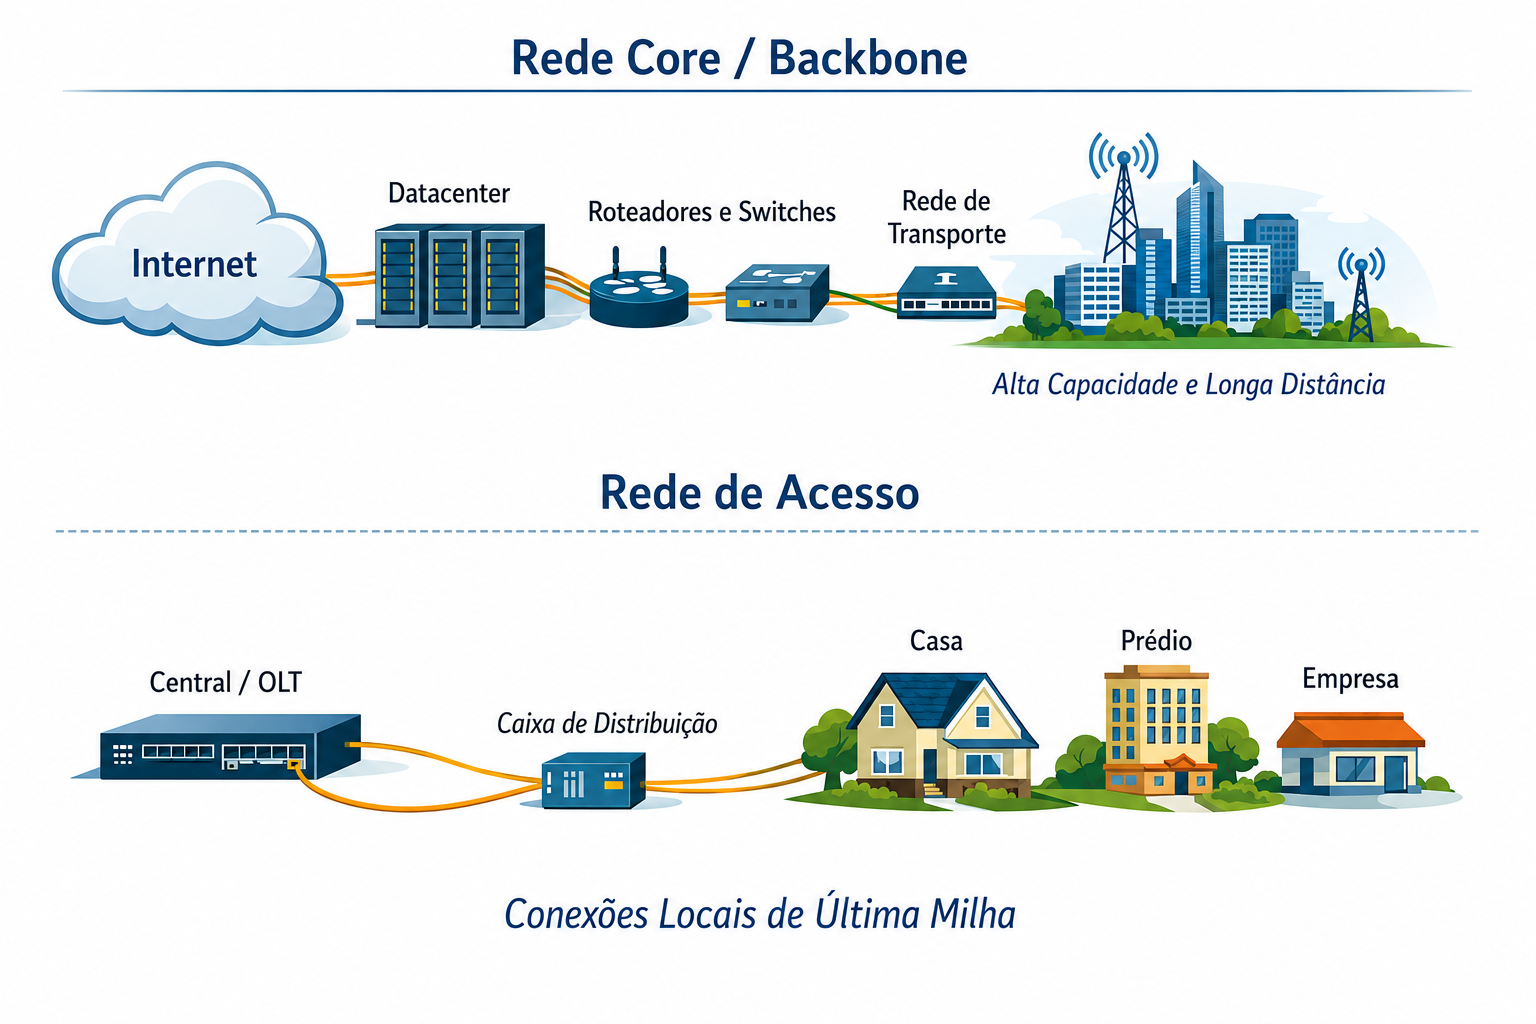
\includegraphics[width=\textwidth]{images/core_acesso.png}
	    \par\footnotesize Fonte: Elaboração própria com auxílio de \gls{ia}.
    }
\end{figure}

Historicamente, as primeiras soluções de acesso à rede de dados foram baseadas em tecnologias discadas sobre a infraestrutura telefônica existente, caracterizadas por baixas taxas de transmissão e forte dependência da qualidade das linhas metálicas. Com o aumento da demanda por serviços de dados, surgiram tecnologias baseadas em par metálico, como as variantes da família xDSL, que permitiram ampliar a capacidade de transmissão utilizando a mesma infraestrutura de cobre da telefonia. Apesar de representarem um avanço significativo em relação ao acesso discado, essas tecnologias apresentaram limitações inerentes ao meio físico, como maior atenuação, suscetibilidade a interferências e forte dependência da distância entre o usuário e a central \cite{tanenbaum2011networks}.

Paralelamente às soluções cabeadas, tecnologias de acesso sem fio também foram amplamente utilizadas. Especialmente em cenários nos quais a implantação de infraestrutura física apresentava restrições econômicas ou geográficas. Sistemas baseados em rádio, redes Wi-Fi de longo alcance e tecnologias celulares possibilitaram ampliar o acesso à conectividade, mostrando-se úteis para expandir a cobertura de serviços em áreas remotas de baixa densidade populacional ou com infraestrutura limitada. Contudo, em muitos casos, essas soluções apresentam limitações relacionadas à capacidade compartilhada, interferências e variabilidade do desempenho. Embora permaneçam relevantes em determinados contextos, o crescimento contínuo do consumo de dados evidenciou a necessidade de meios de acesso com maior capacidade e estabilidade \cite{tanenbaum2011networks}.

Nesse cenário, a fibra óptica passou a ser amplamente reconhecida como a solução mais adequada para redes de acesso de alta capacidade \cite{oliviero2014fiber,keiser2011pon}. Esse meio físico utiliza pulsos de luz para transportar informações ao longo de um filamento de vidro ou plástico de alta pureza, oferecendo vantagens expressivas em relação aos meios metálicos, como elevada largura de banda, menor atenuação do sinal e imunidade a interferências eletromagnéticas \cite{keiser2011pon}. Essas características tornam essa tecnologia especialmente apropriada para atender às exigências atuais e futuras de tráfego, tanto em ambientes residenciais quanto corporativos.

A adoção da fibra óptica no segmento de acesso, possibilitou o surgimento de diferentes modelos de implantação, entre os quais se destaca o \gls{ftth}. O termo \gls{ftth}, refere-se à estratégia de levar a fibra óptica até as dependências do usuário final, seja em residências ou empresas, caracterizando uma rede de acesso totalmente óptica no último trecho da infraestrutura. Essa abordagem elimina as limitações associadas a soluções híbridas ou baseadas em cobre, proporcionando maior desempenho, confiabilidade e escalabilidade para o atendimento às crescentes demandas por serviços de banda larga \cite{oliviero2014fiber}.

Para viabilizar tecnicamente as implantações \gls{ftth} em larga escala, são adotadas arquiteturas de rede específicas, entre as quais se destaca a \gls{pon}. Diferentemente do \gls{ftth}, que define o alcance físico da fibra até o usuário final, a arquitetura \gls{pon} consiste em um padrão arquitetural de rede óptica de acesso baseado na distribuição do sinal em topologia ponto–multiponto por meio de componentes passivos\footnote{Dispositivos que não precisam de energia elétrica}, como fibras e \textit{splitters}, entre a central do provedor e os terminais dos usuários. A ausência de elementos ativos\footnote{Dispositivos que precisam de energia elétrica} no trecho de distribuição contribui para a redução de custos operacionais, aumento da confiabilidade e simplificação da manutenção, tornando a arquitetura \gls{pon} amplamente empregada em redes \gls{ftth} modernas~\cite{keiser2011pon}.

\section{Arquitetura \gls{pon}}

A arquitetura \gls{pon} organiza a rede de acesso a partir de uma topologia ponto-multiponto, na qual um único enlace proveniente da central do provedor é compartilhado entre múltiplos usuários finais. Essa arquitetura fundamenta-se na separação funcional entre elementos ativos e passivos ao longo da infraestrutura, definindo a forma como o sinal óptico é gerado, distribuído e entregue aos assinantes. Em virtude dessa organização, a \gls{pon} se tornou a principal arquitetura empregada na implementação de redes \gls{ftth} em larga escala \cite{itutg9841,keiser2011pon}.

A organização dos elementos que compõem a arquitetura \gls{pon} pode ser visualizada na Figura~\ref{fig:arquitetura_pon}. Observa-se que os componentes ativos concentram-se nas extremidades da rede, com a \gls{olt} localizada na central do provedor e as unidades \gls{onu}/\gls{ont} junto aos usuários finais, enquanto a \gls{odn} é formada exclusivamente por elementos passivos, como fibras ópticas, caixas de emenda e \textit{splitters}. Essa característica de distribuição passiva dispensa alimentação elétrica intermediária ao longo do trecho de atendimento, simplificando a infraestrutura de campo e reduzindo significativamente os pontos potenciais de falha física \cite{keiser2011pon}.

\begin{figure}[htb]
	\caption{Arquitetura de uma rede \gls{pon} baseada em topologia ponto--multiponto}
    \centering
    \parbox{16cm}{
        \centering
        \label{fig:arquitetura_pon}
		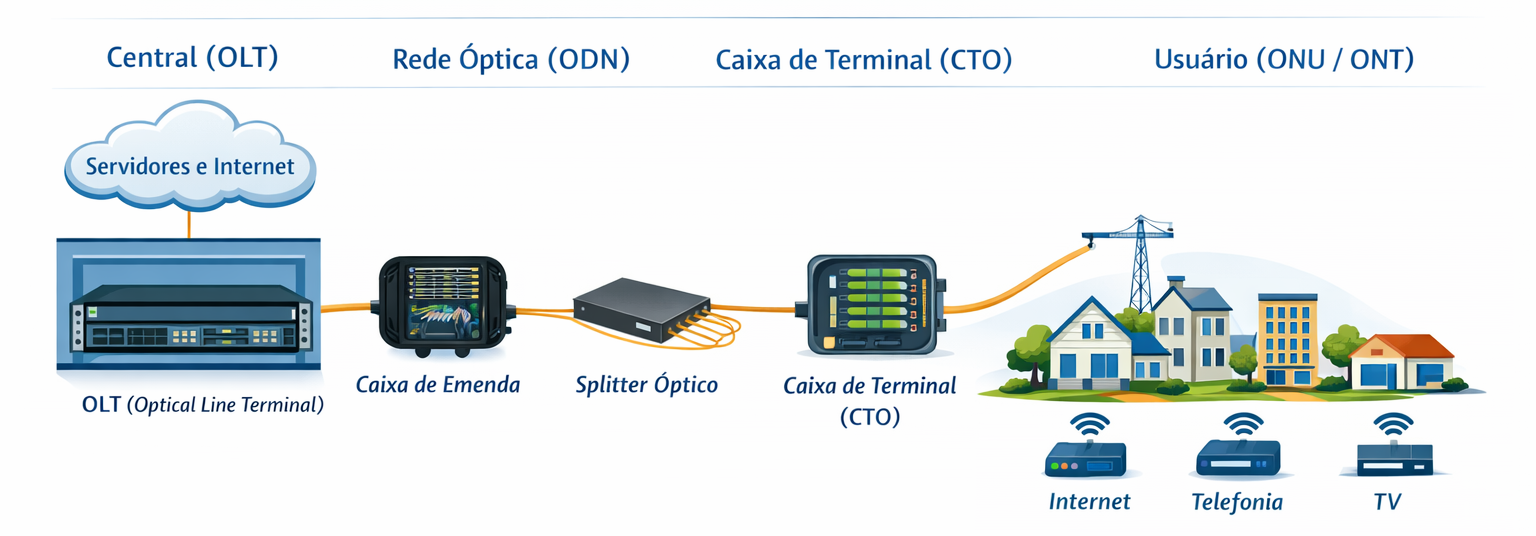
\includegraphics[width=\textwidth]{images/arquitetura_pon.png}
	    \par\footnotesize Fonte: Elaboração própria com auxílio de \gls{ia}.
    }
\end{figure}

A geração inicial do sinal óptico na arquitetura \gls{pon} é realizada por meio de transceptores instalados na \gls{olt}. Esses transceptores, normalmente implementados em módulos do tipo \gls{sfp} ou equivalentes, realizam a conversão do sinal elétrico em óptico e definem parâmetros essenciais da transmissão, como potência de saída, comprimento de onda e sensibilidade de recepção. A partir desses módulos, o sinal gerado é lançado na rede e passa a ser compartilhado entre múltiplos usuários por meio dos componentes passivos da rede de distribuição \cite{keiser2011pon,itutg9842}.

Entre a \gls{olt} (provedor) e as \gls{onu} (clientes) encontra-se a Rede de Distribuição Óptica (\gls{odn}), composta exclusivamente por elementos passivos, como fibras ópticas, \textit{splitters}, caixas de emenda e caixas de terminação. Esses componentes não realizam processamento do sinal nem conversão eletro-óptica, limitando-se à condução e à divisão do sinal luminoso ao longo da topologia da rede. Por ser uma estrutura inteiramente passiva, o desempenho desse trecho da infraestrutura está condicionado estritamente às características físicas de propagação e atenuação dos materiais instalados, o que torna o planejamento e a modelagem matemática dessa seção fatores críticos para a viabilidade técnica \cite{itutg9841,keiser2011pon}. 

As caixas de emenda desempenham papel fundamental na \gls{odn}, sendo utilizadas para a proteção e organização das fusões ópticas entre cabos ao longo do trajeto de distribuição. Essas caixas não realizam atendimento direto aos usuários finais, mas garantem a continuidade do enlace óptico e facilitam a manutenção e possíveis reconfigurações da rede, salvaguardando a integridade das conexões físicas \cite{foa_splice_closure}. Por sua vez, o atendimento aos assinantes ocorre por meio das \gls{cto2},  posicionadas estrategicamente próximas aos usuários e destinadas à conexão dos cabos de derivação (\textit{drop cables}) às unidades finais, organizando o último trecho da rede \gls{ftth} \cite{cto_ftth_distribution,cto_fibracem}.

Embora apresente diversas vantagens, a arquitetura \gls{pon} exige um planejamento criterioso da topologia, da posição dos \textit{splitters} e da distribuição das caixas de emenda e de \gls{cto} ao longo da rede. A divisão excessiva do sinal óptico ou o posicionamento inadequado desses elementos pode comprometer os níveis de potência recebidos pelos usuários finais \cite{keiser2011pon}. Por isso, a análise do orçamento óptico torna-se essencial para garantir o desempenho e a confiabilidade de toda a estrutura. Além dos aspectos relacionados à transmissão de luz, o desempenho e a eficiência geral da rede também estão diretamente associados à forma como sua topologia de distribuição é organizada ao longo da \gls{odn}, influenciando decisões de projeto e o uso da infraestrutura física disponível \cite{keiser2011pon,oliviero2014fiber}.

\section{Topologias Balanceadas e Desbalanceadas em Redes \gls{pon}}

No contexto da arquitetura \gls{pon}, a organização da topologia de distribuição do sinal óptico pode ser classificada, de forma geral, como balanceada ou desbalanceada. Essa classificação está relacionada à forma como o sinal é dividido ao longo da rede e influencia tanto o planejamento lógico quanto a utilização da infraestrutura física disponível \cite{keiser2011pon,itutg9841}.

Em topologias balanceadas, a divisão do sinal ocorre de maneira uniforme entre as diferentes ramificações, resultando em caminhos ópticos com características semelhantes de atenuação e comprimento. Essa abordagem simplifica o planejamento inicial da rede e a validação do orçamento óptico, uma vez que os enlaces tendem a apresentar condições similares de potência recebida. No entanto, esse modelo de distribuição frequentemente demanda um maior número de fibras ópticas ativas ao longo dos cabos de distribuição, pois múltiplas ramificações precisam ser atendidas de forma equivalente desde os níveis iniciais da \gls{odn} \cite{keiser2011pon,oliviero2014fiber}.

Por outro lado, em topologias desbalanceadas, a divisão do sinal é realizada de forma assimétrica, permitindo que determinadas ramificações da rede recebam maior potência óptica ou sejam priorizadas em função da distribuição geográfica dos usuários e da expansão progressiva do atendimento. Em implantações \gls{ftth} reais, essa abordagem é amplamente adotada, pois possibilita maior flexibilidade de projeto e tende a utilizar um número menor de fibras ópticas nos cabos de distribuição, uma vez que nem todos os pontos de atendimento exigem a mesma capacidade ou extensão desde os níveis iniciais da rede \cite{keiser2011pon}.

\begin{figure}[htb]
	\caption{Comparação entre topologias balanceada e desbalanceadas em redes \gls{pon}}
	\label{fig:topologias_pon}
    \centering
    \parbox{16cm}{
		\centering
		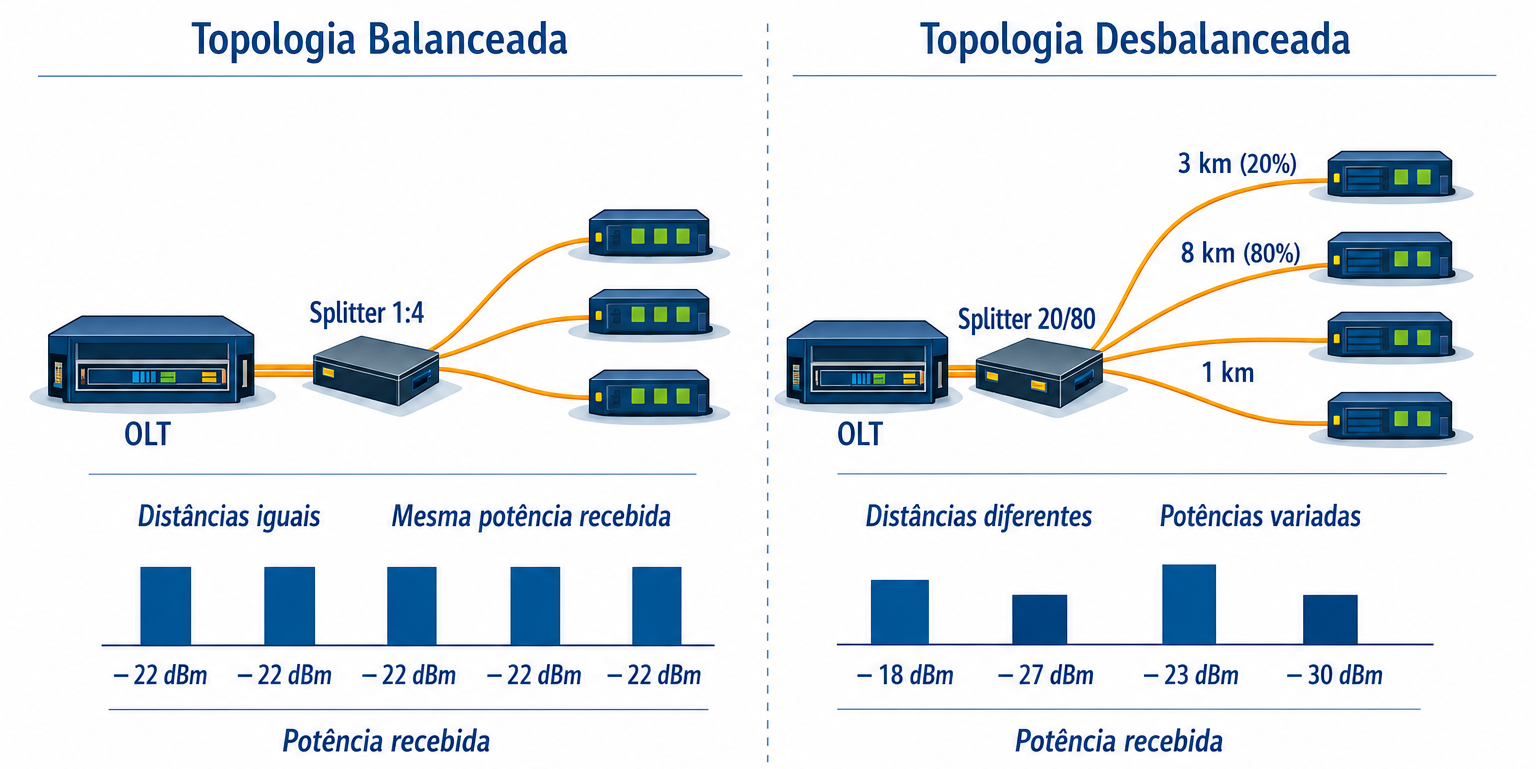
\includegraphics[width=\textwidth]{images/topologias_pon.png}
		\par\footnotesize Fonte: Elaboração própria com auxílio de \gls{ia}.
    }
\end{figure}

A distinção entre as abordagens balanceada e desbalanceadasa em redes \gls{pon} pode ser observada na Figura~\ref{fig:topologias_pon}. No modelo balanceado, as ramificações apresentam extensões semelhantes, resultando em níveis de potência recebida praticamente equivalentes nos terminais finais, o que simplifica o planejamento e a validação do orçamento óptico. Em contrapartida, na distribuição desbalanceada, os enlaces possuem comprimentos distintos, ocasionando diferentes níveis de atenuação e, consequentemente, potências recebidas variáveis, o que permite maior flexibilidade no projeto da rede, porém exige uma análise individualizada do orçamento óptico para cada ramificação \cite{keiser2011pon}.

Dessa forma, a escolha entre topologias balanceadas e desbalanceadas envolve um compromisso entre simplicidade de planejamento, balanceamento de potência e eficiência no uso da infraestrutura física. Independentemente da topologia adotada, torna-se essencial avaliar o orçamento óptico de forma adequada para cada ramificação final, garantindo que todos os enlaces atendam aos limites operacionais estabelecidos pelos equipamentos ativos utilizados \cite{apnic_gpon_budget}. Além da organização topológica da rede, a arquitetura \gls{pon} também é definida pelos padrões tecnológicos adotados, os quais estabelecem limites de capacidade e de divisão do sinal, influenciando diretamente o dimensionamento da rede de acesso \cite{itutg9841,itu_optical_access_tutorial}.

\section{Padrões \gls{pon} e Capacidade de Divisão}

Diversos padrões de redes ópticas passivas são utilizados em implantações \gls{ftth}, entre os quais se destacam \gls{epon}, \gls{gpon}, \gls{xgpon} e \gls{xgspon}. Eles se diferem principalmente em aspectos como taxas de transmissão, comprimentos de onda utilizados e capacidade de atendimento. Entretanto, independentemente do padrão adotado, o princípio fundamental da arquitetura \gls{pon} permanece o mesmo.\cite{keiser2011pon,itutg9841}.

Do ponto de vista do planejamento do orçamento, é importante destacar que a metodologia de cálculo é conceitualmente idêntica para todos os padrões \gls{pon}. Em todos os casos, a margem é determinada pela diferença entre a potência de transmissão do equipamento de origem e a sensibilidade mínima de recepção do terminal, considerando-se as perdas acumuladas ao longo do caminho. Assim, a tecnologia \gls{pon} adotada não altera a lógica matemática da rede, mas define os limites e parâmetros operacionais dentro dos quais esse cálculo deve ser realizado \cite{keiser2011pon,holight_optical_budget}.

As principais diferenças entre os padrões \gls{pon} refletem-se nos limites normativos associados à capacidade do sistema, especialmente na taxa máxima de divisão do sinal suportada pela arquitetura. Esse parâmetro influencia diretamente o número máximo de ramificações que podem ser atendidas por uma única porta da \gls{olt}, impactando decisões de projeto relacionadas à topologia física, à distribuição dos \textit{splitters} e à densidade de atendimento \cite{itutg9841,itu_optical_access_tutorial}.

A Tabela~\ref{tab:padroes_pon_divisao} apresenta uma relação entre alguns dos principais padrões \gls{pon} e as taxas máximas típicas de divisão adotadas em projetos de redes \gls{ftth}, conforme práticas amplamente referenciadas na literatura técnica e em recomendações normativas \cite{itutg9841,keiser2011pon,itu_optical_access_tutorial}.

\begin{table}[htb]
\centering
\caption{Padrões \gls{pon} e taxas máximas típicas de divisão}
\label{tab:padroes_pon_divisao}
\begin{tabular}{c c}
\hline
\textbf{Padrão \gls{pon}} & \textbf{Taxa máxima típica de divisão} \\
\hline
Epon      & até 1$\times$64 \\
Gpon      & até 1$\times$128 \\
XG-pon    & até 1$\times$128 \\
XGS-pon   & até 1$\times$128 \\
\hline
\end{tabular}
\par\footnotesize Fonte: Adaptado de \cite{itutg9841} e \cite{keiser2011pon}.
\end{table}

A capacidade de divisão do sinal óptico varia de acordo com a tecnologia \gls{pon} adotada, conforme ilustrado na Figura~\ref{fig:epon_gpon_divisao}. No padrão \gls{epon}, uma única fibra pode ser compartilhada entre até 64 usuários finais, enquanto na arquitetura \gls{gpon} essa capacidade é ampliada, possibilitando a divisão do sinal para até 128 clientes. Essa diferença de escala determina a concentração de assinantes por porta física na central, definindo o nível de compartilhamento do meio físico e orientando a distribuição geográfica dos elementos passivos de derivação \cite{itutg9841,itu_optical_access_tutorial}.

\begin{figure}[htb]
	\caption{Comparação entre os padrões \gls{epon} e \gls{gpon} quanto à capacidade de divisão}
    \centering
    \parbox{16cm}{
		\centering
        \label{fig:epon_gpon_divisao}
		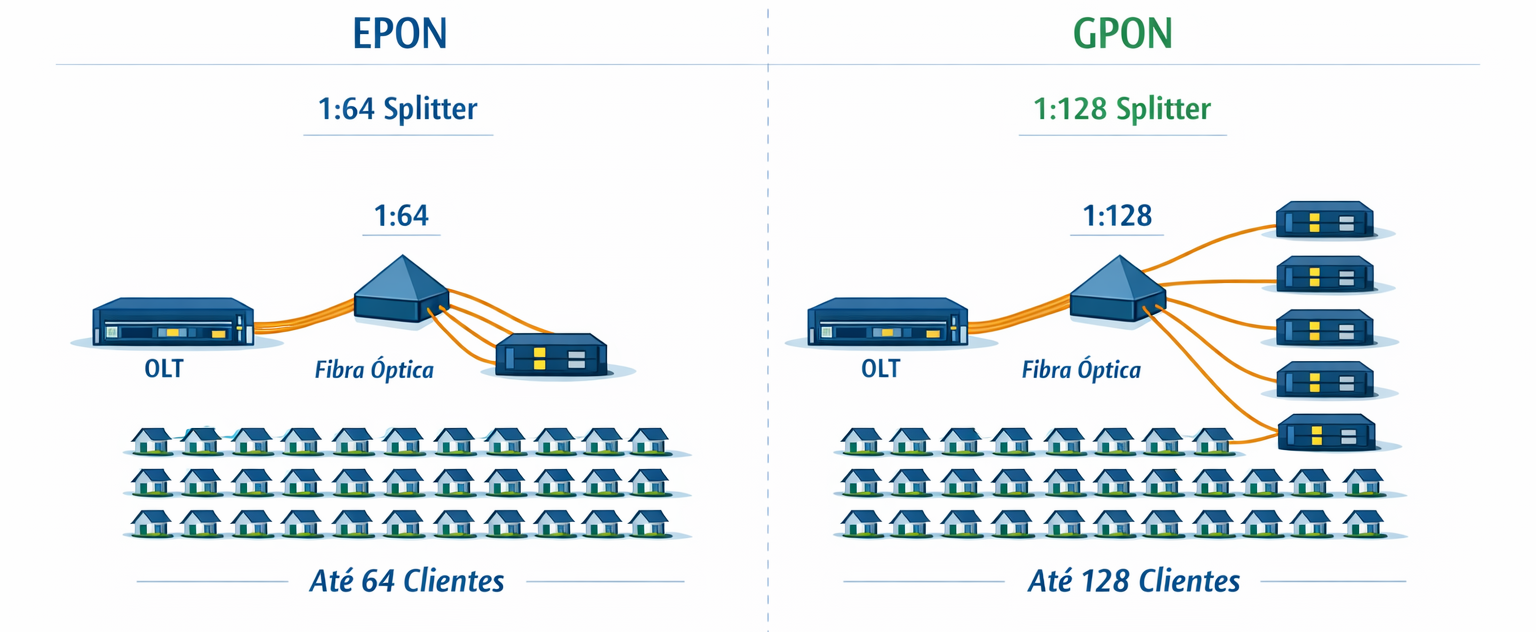
\includegraphics[width=\textwidth]{images/epon_gpon_divisao.png}
		\par\footnotesize Fonte: Elaboração própria com auxílio de \gls{ia}.
    }
\end{figure}

Dessa forma, a escolha da tecnologia \gls{pon} está associada principalmente à capacidade de atendimento e aos limites arquiteturais da infraestrutura, enquanto o cálculo do orçamento óptico permanece baseado nos mesmos fundamentos físicos. Essa característica reforça a importância de abordagens de planejamento que permitam a parametrização do padrão tecnológico adotado, possibilitando avaliar diferentes cenários de divisão e expansão do atendimento sem alterar a lógica fundamental do cálculo do orçamento \cite{keiser2011pon,holight_optical_budget}.

\section{Orçamento Óptico em Redes \gls{pon}}

O orçamento constitui um dos aspectos centrais no planejamento de redes baseadas na arquitetura \gls{pon}, pois está diretamente relacionado à garantia de que o sinal chegue ao usuário final dentro dos níveis adequados de potência. Em infraestruturas \gls{ftth}, nas quais o sinal é compartilhado entre múltiplos assinantes por meio de componentes passivos, a correta avaliação das perdas ao longo do enlace torna-se essencial para assegurar o desempenho e a confiabilidade do sistema \cite{keiser2011pon}. Nesse contexto, a análise do orçamento envolve a consideração de fatores como os limites de potência definidos pelos transceptores, a atenuação da fibra óptica, as perdas introduzidas por dispositivos passivos e conexões, bem como critérios normativos associados à transmissão.

Do ponto de vista físico, essa análise pode ser estruturada seguindo o percurso do sinal desde sua geração nos transceptores da \gls{olt} até a recepção nas unidades terminais, considerando-se, ao longo do trajeto, as perdas acumuladas pelos diferentes elementos da infraestrutura \cite{keiser2011pon,apnic_gpon_budget}.

\begin{figure}[htb]
	\caption{Consolidação das perdas no enlace óptico em redes \gls{pon}}
	\label{fig:perdas_consolidadas_enlace}
    \centering
    \parbox{16cm}{
		\centering
		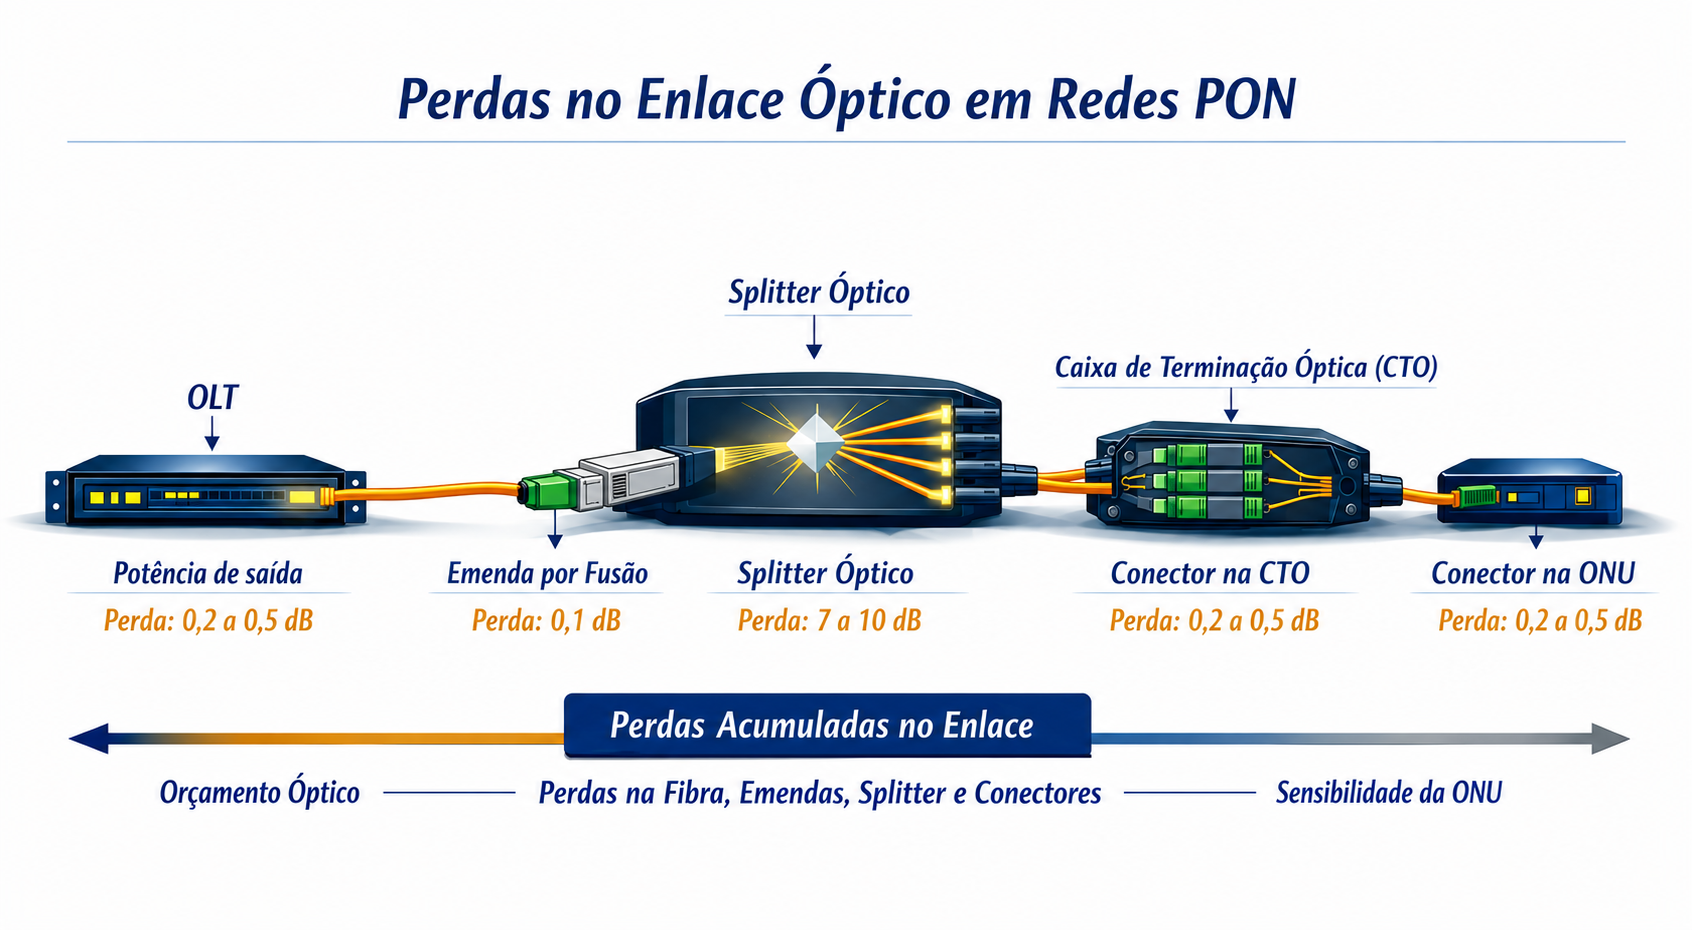
\includegraphics[width=\textwidth]{images/perdas_consolidadas_enlace.png}
		\par\footnotesize Fonte: Elaboração própria com auxílio de \gls{ia}.
    }
\end{figure}

A Figura~\ref{fig:perdas_consolidadas_enlace} apresenta uma visão global das atenuações incidentes ao longo de um enlace típico em redes \gls{pon}. Observa-se que a atenuação total resulta da soma de perdas distribuídas na fibra óptica e das perdas concentradas introduzidas por emendas, \textit{splitters} e conectores presentes na \gls{olt}, nas caixas de terminação e nas unidades \gls{onu}. A consolidação desses fatores é fundamental para a verificação do orçamento, uma vez que o enlace somente será considerado viável se a potência recebida no terminal final permanecer acima de sua sensibilidade mínima especificada \cite{keiser2011pon,holight_optical_budget}.

De forma conceitual, o orçamento pode ser entendido como a diferença entre a potência de transmissão (\textit{Tx}) e a sensibilidade mínima do receptor (\textit{Rx}), representando a perda máxima admissível para que o enlace permaneça ativo \cite{holight_optical_budget}. Em termos práticos, a validação do enlace é realizada comparando a capacidade de tolerar perdas com a perda total do caminho, que resulta da soma das atenuações introduzidas por componente ao longo do trajeto \cite{apnic_gpon_budget}. Quando a perda total excede a margem disponível, a potência recebida tende a ficar abaixo do limiar necessário e o enlace pode apresentar degradação de desempenho ou falhas de conexão \cite{holight_optical_budget}.

\subsection{Classes Ópticas e Transceptores \gls{pon}}

Os sistemas \gls{pon} utilizam transceptores instalados na \gls{olt} e nas unidades terminais (\gls{onu}/\gls{ont}) para realizar a transmissão e a recepção dos sinais. Esses componentes são normalmente implementados em módulos do tipo \gls{sfp} ou \gls{gbic}, que integram os elementos responsáveis pela emissão do feixe luminoso e pela detecção do sinal recebido. As características desses módulos, em especial a potência de transmissão (\textit{Tx}) e a sensibilidade de recepção (\textit{Rx}), exercem influência direta sobre a margem de atenuação disponível no enlace \cite{keiser2011pon,itutg9842}.

Nas redes \gls{gpon}, os transceptores são classificados em diferentes categorias de desempenho, como B+, C+ e C++, conforme definidas pelas recomendações da ITU-T \cite{itutg9842}. Cada classe estabelece limites mínimos de potência de transmissão e máximos de sensibilidade de recepção, determinando, assim, a perda total máxima admissível entre a \gls{olt} e as \gls{onu}. Dessa forma, a especificação adotada impõe restrições diretas à extensão máxima da rede, à taxa de divisão do sinal e à complexidade da topologia que pode ser suportada \cite{itutg9841,itutg9842}.

A Tabela~\ref{tab:classes_opticas_gpon} apresenta valores típicos de potência de transmissão, sensibilidade de recepção e margem de atenuação associados às principais classes de tranceptores utilizadas em sistemas \gls{gpon}, amplamente adotados como referência no planejamento de redes \gls{ftth} \cite{apnic_gpon_budget}.

\begin{table}[htb]
\centering
\caption{Classes ópticas \gls{gpon} e parâmetros típicos}
\label{tab:classes_opticas_gpon}
\begin{tabular}{c c c c}
\hline
\textbf{Classe óptica} & \textbf{Tx mín. (dBm)} & \textbf{Rx mín. (dBm)} & \textbf{Orçamento típico (dB)} \\
\hline
B+  & +1,5  & -28  & 29,5 \\
C+  & +3,0  & -32  & 35 \\
C++ & +5,0  & -35  & 40 \\
\hline
\end{tabular}
\par\footnotesize Fonte: Elaborado pelo autor com base em \cite{apnic_gpon_budget} e \cite{holight_optical_budget}.
\end{table}

Conforme apresentado na Tabela~\ref{tab:classes_opticas_gpon}, classes mais elevadas disponibilizam maior orçamento óptico, suportando enlaces mais longos, maiores taxas de divisão e topologias mais complexas, incluindo configurações com múltiplos estágios de \textit{splitters} ou topologias desbalanceadas. Por outro lado, os transceptores dessas classes apresentam maior custo, tornando a escolha uma decisão de projeto que envolve o equilíbrio entre desempenho técnico e viabilidade econômica \cite{keiser2011pon}.

\begin{figure}[htb]
	\caption{Conexão do transceptor óptico à porta \gls{sfp} da \gls{olt}}
	\label{fig:transceiver_sfp_olt}
    \centering
    \parbox{16cm}{
		\centering
		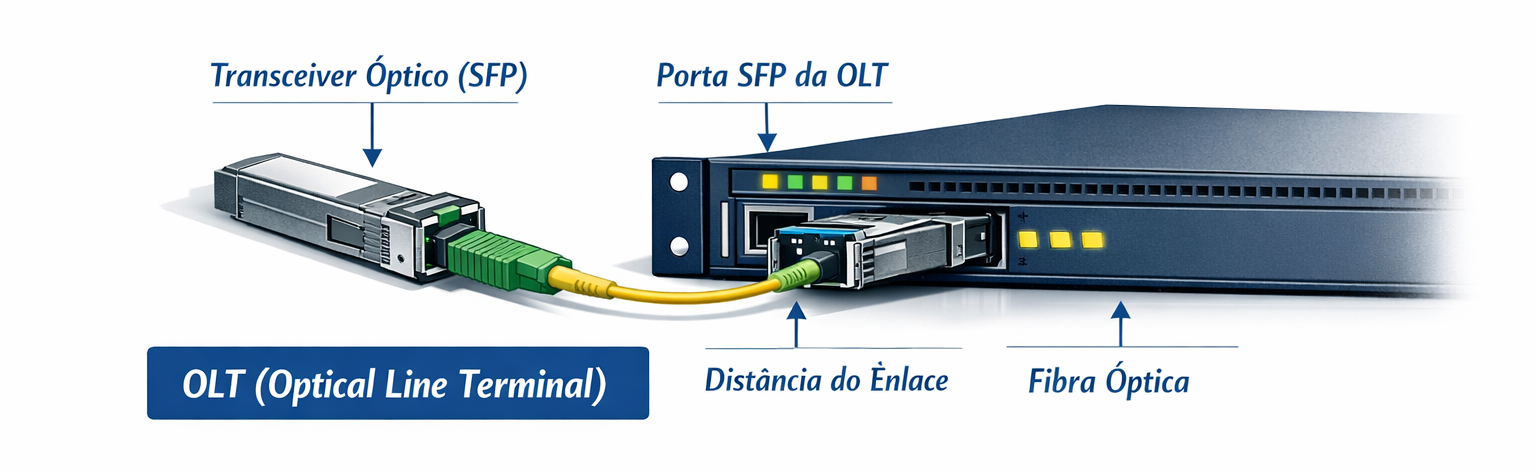
\includegraphics[width=\textwidth]{images/transceiver_sfp_olt.png}
		\par\footnotesize Fonte: Elaboração própria com auxílio de \gls{ia}.
    }
\end{figure}

A geração do sinal luminoso em redes \gls{pon} ocorre na \gls{olt} por meio de transceptores conectados às suas portas do tipo \gls{sfp}, conforme ilustrado na Figura~\ref{fig:transceiver_sfp_olt}. Esses módulos são responsáveis pela conversão do sinal elétrico em óptico, além de definirem parâmetros essenciais da transmissão, como potência de saída, comprimento de onda e alcance máximo do enlace. A partir do transceptor, o sinal é acoplado à fibra e lançado na \acrlong{odn}, dando início ao processo de atendimento aos usuários finais.

No contexto do planejamento de redes \gls{ftth}, a correta consideração da classe do transceptor é fundamental para garantir que o orçamento calculado seja compatível com os limites operacionais dos equipamentos utilizados. Assim, a definição adequada da classe selecionada, em conjunto com a modelagem das perdas ao longo da rede, constitui um elemento central para a validação técnica e a confiabilidade do projeto da rede \gls{pon}. Neste trabalho, esses valores são apresentados como referência teórica; o protótipo permite informar diretamente a potência de transmissão e a sensibilidade de recepção de cada equipamento, sem selecionar automaticamente uma classe normativa.

\subsection{Perdas Distribuídas: Atenuação da Fibra Óptica}

A atenuação total em um enlace \gls{pon} pode ser organizada em perdas distribuídas e concentradas. As primeiras estão associadas principalmente à atenuação natural do sinal na fibra óptica e variam conforme o comprimento de onda e as características do cabo, conforme descrito em recomendações técnicas \cite{itutg652_2024}. 

No caso da atenuação da fibra, especificações técnicas associadas indicam limites típicos de atenuação, como valores em torno de 0{,}30~dB/km  \cite{prysmian_g652d_datasheet}. Assim, o comprimento do enlace e a faixa de operação impactam diretamente o orçamento, tornando necessário planejar trajetos coerentes com a infraestrutura instalada e com as metas de divisão do sinal \cite{itutg652_2024}.

\begin{figure}[htb]
	\caption{Atenuação do sinal ao longo da fibra óptica em função da distância}
	\label{fig:atenuacao_fibra}
    \centering
    \parbox{16cm}{
		\centering
		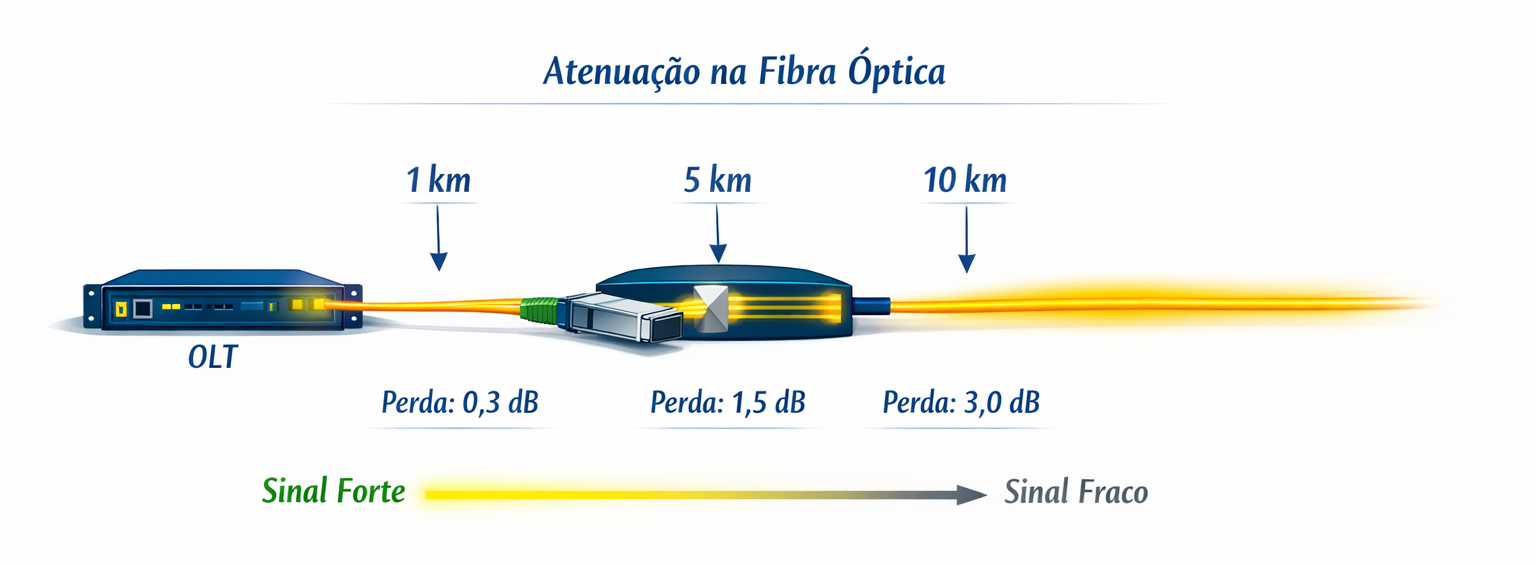
\includegraphics[width=\textwidth]{images/atenuacao_fibra.png}
		\par\footnotesize Fonte: Elaboração própria com auxílio de \gls{ia}.
    }
\end{figure}

A atenuação constitui uma perda distribuída ao longo do enlace, crescendo proporcionalmente ao comprimento do cabo empregado. Essa relação pode ser observada na Figura~\ref{fig:atenuacao_fibra}, na qual se evidencia que, à medida que a distância aumenta, ocorre a redução progressiva da potência do sinal. Em projetos de redes \gls{pon}, essa atenuação natural representa um dos fatores fundamentais no cálculo do orçamento óptico, devendo ser considerada conjuntamente com as perdas introduzidas por conectores, emendas e \textit{splitters}.

\subsection{Perdas Concentradas: \textit{Splitters}}

A divisão do sinal na arquitetura \gls{pon} é realizada por meio de \textit{splitters}, inseridos ao longo da \acrlong{odn}, conforme ilustrado na Figura~\ref{fig:splitter_optico }. Esses dispositivos recebem a portadora proveniente da \gls{olt} por uma única fibra de entrada e realizam a divisão da potência em múltiplas saídas, distribuindo o sinal para diferentes ramificações. Por se tratarem de elementos totalmente passivos, os \textit{splitters} não requerem alimentação elétrica e contribuem para a redução de custos operacionais e o aumento da confiabilidade dos sistemas de acesso \gls{pon}.

\begin{figure}[htb!]
	\caption{Funcionamento do \textit{splitter} e divisão do sinal em redes \gls{pon}}
	\label{fig:splitter_optico }
    \centering
    \parbox{16cm}{
		\centering
		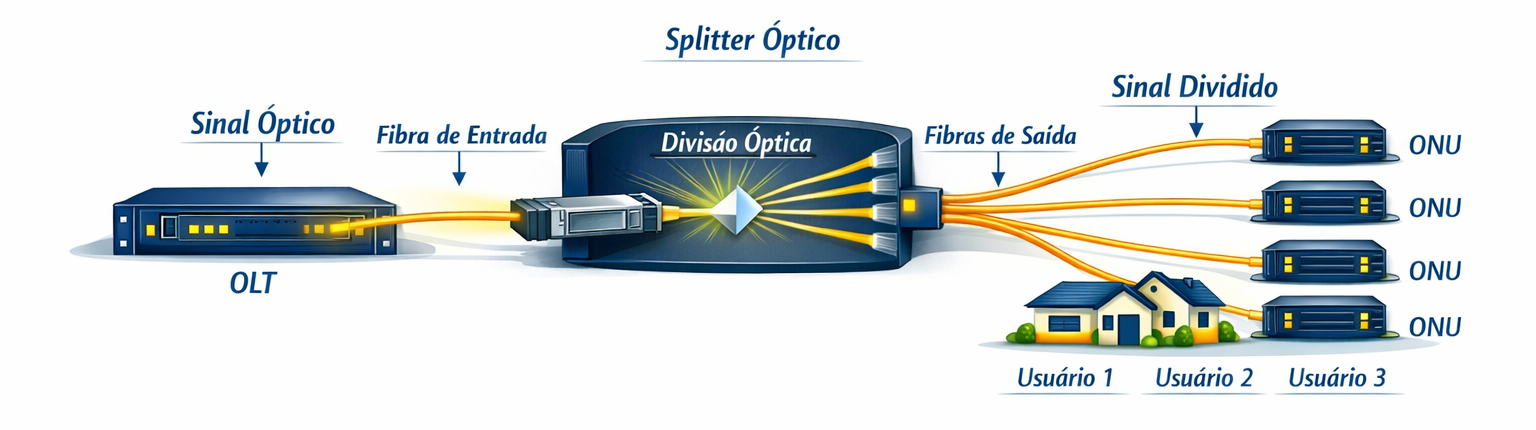
\includegraphics[width=\textwidth]{images/splitter_optico.png}
		\par\footnotesize Fonte: Elaboração própria com auxílio de \gls{ia}.
    }
\end{figure}

Entre os componentes passivos, os \textit{splitters} geralmente representam a maior parcela da atenuação em redes \gls{pon}, uma vez que realizam a divisão do sinal em múltiplas derivações ao longo da rede de distribuição. Em projetos \gls{ftth}, a perda introduzida por esses componentes tende a superar as perdas associadas a conectores e emendas, tornando-se um fator determinante no dimensionamento do enlace \cite{keiser2011pon,apnic_gpon_budget}.

A perda na inserção de um \textit{splitter} está diretamente relacionada à sua razão de derivação. Em configurações balanceadas, o sinal é distribuído de forma uniforme entre todas as saídas, resultando em perdas semelhantes em cada ramificação. Já em configurações desbalanceadas, a divisão ocorre de forma assimétrica, permitindo priorizar determinados caminhos da rede, porém introduzindo níveis distintos de atenuação entre as saídas, o que exige uma análise individualizada do orçamento para cada ramificação final \cite{keiser2011pon}.

A Tabela~\ref{tab:perdas_splitters} apresenta valores típicos de perda de inserção para diferentes configurações de \textit{splitters}, incluindo divisões balanceadas e desbalanceadas, amplamente utilizadas como referência no planejamento de redes \gls{pon} \cite{apnic_gpon_budget,holight_optical_budget}.

\begin{table}[ht!]
\centering
\caption{Perdas típicas de inserção de \textit{splitters} ópticos em redes \gls{pon}}
\label{tab:perdas_splitters}
\begin{tabular}{c c c}
\hline
\textbf{Splitter} & \textbf{Tipo de divisão} & \textbf{Perda típica (dB)} \\
\hline
1$\times$2   & Balanceada     & 3,5 \\
1$\times$4   & Balanceada     & 7,2 \\
1$\times$8   & Balanceada     & 10,5 \\
1$\times$16  & Balanceada     & 13,7 \\
\hline
10/90 & Desbalanceada & $\approx$ 10,5 / 1,5 \\
20/80 & Desbalanceada & $\approx$ 7,8 / 3,8 \\
30/70 & Desbalanceada & $\approx$ 6,3 / 5,5 \\
40/60 & Desbalanceada & $\approx$ 4,7 / 6,8 \\
\hline
\end{tabular}
\end{table} 

Os valores apresentados na Tabela~\ref{tab:perdas_splitters} representam perdas típicas utilizadas como referência no planejamento de redes \gls{ftth}. Em especial, os \textit{splitters} desbalanceados introduzem níveis distintos de atenuação entre as saídas, o que permite flexibilizar o projeto da rede, mas exige que o orçamento seja calculado individualmente para cada ramal. Assim, a correta modelagem das perdas associadas aos \textit{splitters} é fundamental para garantir que todos os enlaces atendam aos limiares de sensibilidade estabelecidos para os terminais ativos do projeto.

\subsection{Perdas Concentradas: Conectores e Emendas}

Além da atenuação distribuída ao longo do meio físico, o orçamento óptico em redes \gls{pon} é influenciado por perdas concentradas introduzidas por conexões e emendas, conforme ilustrado na Figura~\ref{fig:perdas_conexoes_emendas}. Cada conector  presente na \gls{olt}, nas caixas de terminação e nas \glspl{onu} contribui com perdas adicionais, tipicamente na faixa de 0,2 a 0,5~dB, enquanto as emendas por fusão inseridas ao longo da fibra apresentam atenuações menores individualmente, porém relevantes quando acumuladas. 

\begin{figure}[ht!]
	\caption{Perdas introduzidas por conexões e emendas na rede \gls{pon}}
	\label{fig:perdas_conexoes_emendas}
    \centering
    \parbox{16cm}{
		\centering
		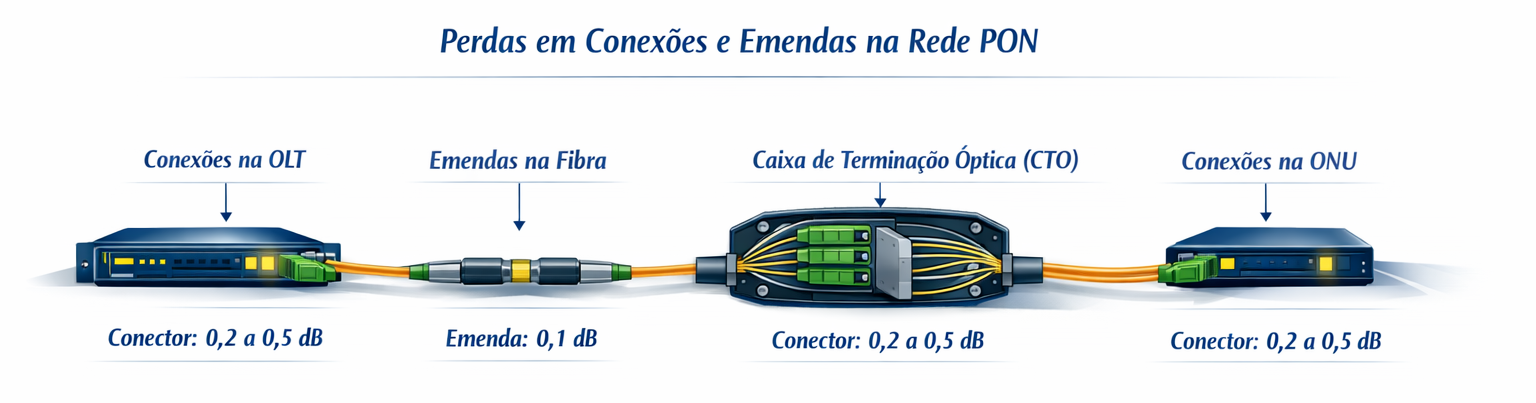
\includegraphics[width=\textwidth]{images/perdas_conexoes_emendas.png}
		\par\footnotesize Fonte: Elaboração própria com auxílio de \gls{ia}.
    }
\end{figure}

Dessa forma, a quantidade de interconexões e fusões realizadas em campo passa a ser um fator importante na previsão de desempenho do canal, reforçando a necessidade de planejamento criterioso da infraestrutura de distribuição. Além das perdas introduzidas pelos componentes passivos ao longo do trajeto, a viabilidade do projeto também depende diretamente das características dos equipamentos utilizados, em especial da potência de transmissão e da sensibilidade de recepção dos transceptores instalados na \gls{olt} e nas \gls{onu}.

A análise do orçamento óptico, embora fundamentada em princípios bem estabelecidos, envolve a consideração simultânea de diversos parâmetros técnicos e da interação entre múltiplos elementos ao longo do enlace. Em projetos reais de sistemas \gls{pon}, especialmente em implantações \gls{ftth} de maior escala, a quantidade de componentes, variações topológicas e diferentes cenários de expansão tornam esse processo progressivamente mais complexo. Nesse contexto, a forma como essa margem de transmissão é calculada, documentada e validada passa a exercer influência direta sobre a confiabilidade do projeto, motivando o uso de ferramentas e métodos específicos para apoiar o planejamento dessas redes.

\section{Ferramentas e Métodos Atuais de Planejamento}

O planejamento de redes ópticas \gls{pon} é atualmente realizado com o auxílio de diferentes ferramentas e métodos, que variam desde abordagens essencialmente manuais até soluções computacionais mais especializadas. Em geral, esses recursos são empregados para estimar o orçamento de potência, definir a topologia física e organizar a distribuição dos componentes ao longo do enlace. Apesar de contribuírem para o processo de projeto, muitas dessas abordagens apresentam limitações relacionadas à integração entre cálculo técnico e representação visual da rede, à flexibilidade na modelagem da topologia e à dependência de intervenções manuais, fatores que podem comprometer a eficiência do dimensionamento de sistemas \gls{ftth} \cite{keiser2011pon,munzner2014visualization}. 

Uma prática amplamente adotada no planejamento de redes \gls{pon} consiste na utilização de planilhas eletrônicas para o cálculo do orçamento. Nessas planilhas, são inseridos manualmente parâmetros como distâncias de fibra, perdas associadas a conectores, fusões e dispositivos passivos, bem como margens de segurança definidas pelo projetista. Embora essa abordagem viabilize as estimativas necessárias, ela depende fortemente da correta inserção dos dados e da interpretação manual dos resultados, o que torna o processo suscetível a inconsistências, especialmente em projetos com múltiplos componentes distribuídos geograficamente \cite{keiser2011pon}. 

Além das planilhas, o planejamento da topologia da rede é frequentemente realizado por meio de diagramas manuais ou ferramentas genéricas de desenho, que auxiliam a organização dos elementos e suas interconexões. Esse tipo de representação costuma não estar integrado ao cálculo, exigindo manutenção paralela entre documentação visual e planilhas de perdas, o que tende a aumentar retrabalho quando a topologia sofre alterações ao longo do projeto.

Paralelamente, observa-se o uso de soluções de georreferenciamento (\gls{gis}) para o planejamento e, principalmente, para a documentação e operação de redes \gls{ftth}. Estudos e relatos técnicos descrevem abordagens nas quais o \gls{gis} é empregado para mapear rotas, distribuir elementos, além de manter registros georreferenciados da infraestrutura instalada, favorecendo documentação e gestão operacional \cite{chakali2025gis_ftth,vargas2025gis_ecuador,irjet2017ftth_gis_autocad,qgis2016ftth_case}. Esse enfoque é particularmente útil para inventário e manutenção, pois consolida a localização física de cabos, caixas, rotas e pontos de acesso em um ambiente espacial.

Entretanto, do ponto de vista da compreensão lógica da rede \gls{pon}, é comum que soluções orientadas ao registro geográfico privilegiem a representação dos ativos a partir do mapa e do cadastro de componentes (cabos, caixas, \textit{splitters} e fusões), com navegação por camadas e consultas por localização \cite{chakali2025gis_ftth,vargas2025gis_ecuador}. Nessa perspectiva, a visualização pode enfatizar ``onde'' os elementos estão e ``o que'' está cadastrado, mas nem sempre favorece uma leitura lógica integrada do encadeamento completo da rede, desde a \gls{olt} até os pontos finais de atendimento, especialmente quando o usuário precisa compreender rapidamente as ligações entre os elementos em diferentes níveis da topologia.

Em alguns sistemas de inventário, a própria documentação do fabricante descreve a existência de representações de rede que combinam inventário físico e lógico e permitem a análise de circuitos e topologias, indicando que o tema de integração entre camadas é relevante na prática \cite{servicenow_inventory_2024}. Ainda assim, quando a visualização permanece predominantemente geográfica, tende a ser mais comum a inspeção de elementos por localidade (por exemplo, detalhes de caixas, emendas e terminais acessados a partir do mapa) do que uma representação lógica global de todas as conexões \gls{pon} de ponta a ponta.

De modo geral, a fragmentação entre cálculo, documentação geográfica e representação lógica pode dificultar a identificação de inconsistências e a análise do impacto de alterações na topologia. Nesse contexto, torna-se relevante considerar abordagens que integrem diferentes etapas do planejamento \cite{munzner2014visualization,keiser2011pon}.

A Figura~\ref{fig:comparacao_planejamento} ilustra essa diferença, comparando o processo manual, caracterizado por etapas independentes e suscetíveis a erros, com o uso de ferramentas integradas, que proporcionam automação, centralização das informações e maior confiabilidade na análise do projeto.

\begin{figure}[htb]
	\caption{Comparação entre o planejamento manual e o uso de ferramentas integradas no projeto de redes ópticas}
	\label{fig:comparacao_planejamento}
    \centering
    \parbox{16cm}{
		\centering
		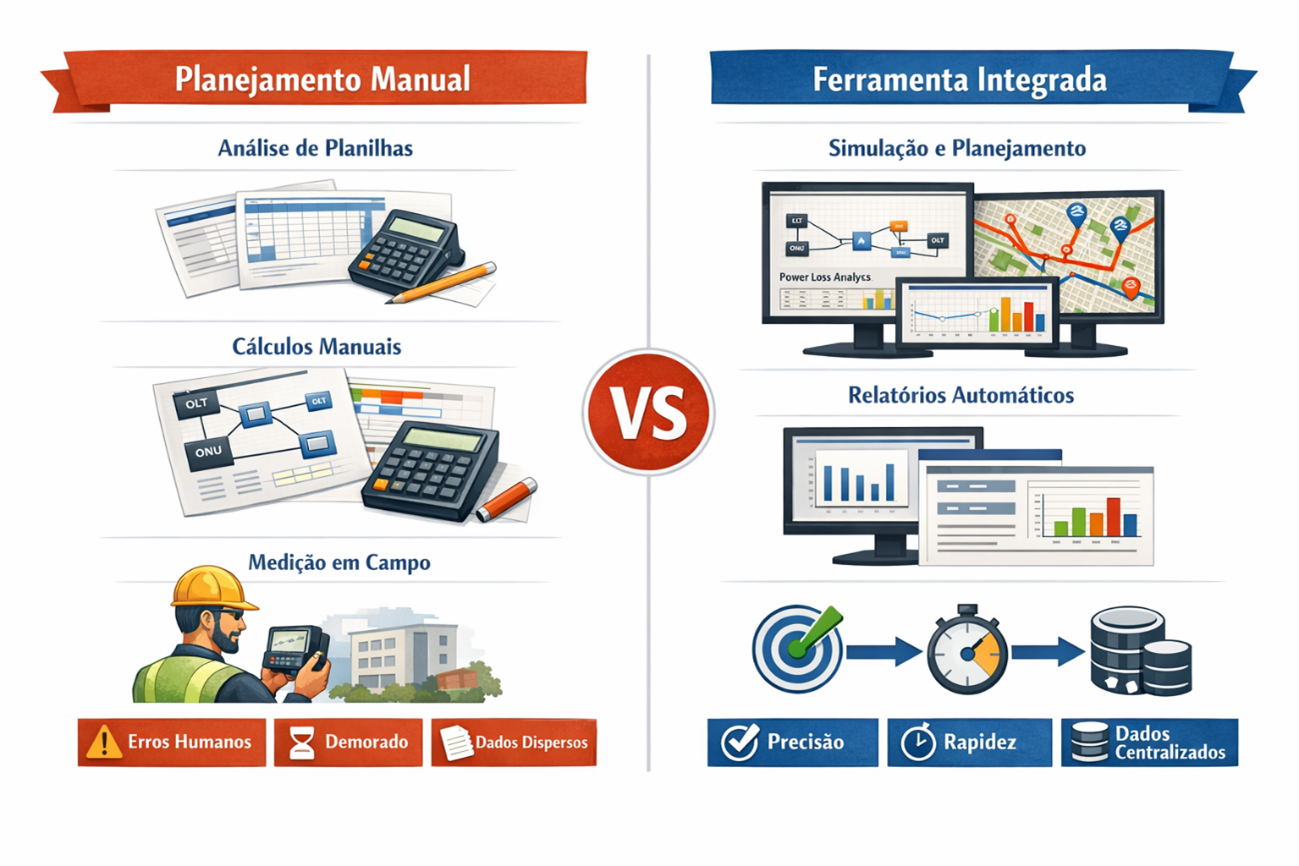
\includegraphics[width=\textwidth]{images/comparacao_planejamento.png}
		\par\footnotesize Fonte: Elaboração própria com auxílio de \gls{ia}.
    }
\end{figure}

\section{Visualização de Dados em Sistemas Complexos}

Sistemas complexos caracterizam-se pela presença de múltiplos elementos interconectados, cujas relações não podem ser plenamente compreendidas por meio da análise isolada de cada componente. Nesses sistemas, o comportamento global emerge a partir da interação entre as partes, tornando a interpretação baseada apenas em dados tabulares ou descrições textuais limitada. Nesse contexto, a visualização de dados assume um papel fundamental como instrumento de apoio à cognição, permitindo transformar informações abstratas em representações que favorecem a compreensão, a análise e a tomada de decisão \cite{card1999information,ware2013information}.

A visualização de dados não se restringe à apresentação estética da informação, mas atua como um meio de ampliar as capacidades cognitivas do usuário. Conforme discutido por \citeonline{card1999information}, representações visuais bem projetadas reduzem a carga cognitiva, facilitam a identificação de padrões e tornam explícitas as relações que seriam difíceis de perceber em formatos tradicionais. Em sistemas com grande volume de dados e múltiplas dependências, como redes de telecomunicações, essa exibição passa a ser um elemento essencial para compreender a estrutura e o funcionamento do sistema como um todo.

\begin{figure}[htb]
	\caption{Processo de visualização de dados em sistemas complexos, desde a coleta e integração de dados até a geração de \textit{insights} para apoio à tomada de decisão}
	\label{fig:visualizacao_sistemas_complexos}
    \centering
    \parbox{16cm}{
		\centering
		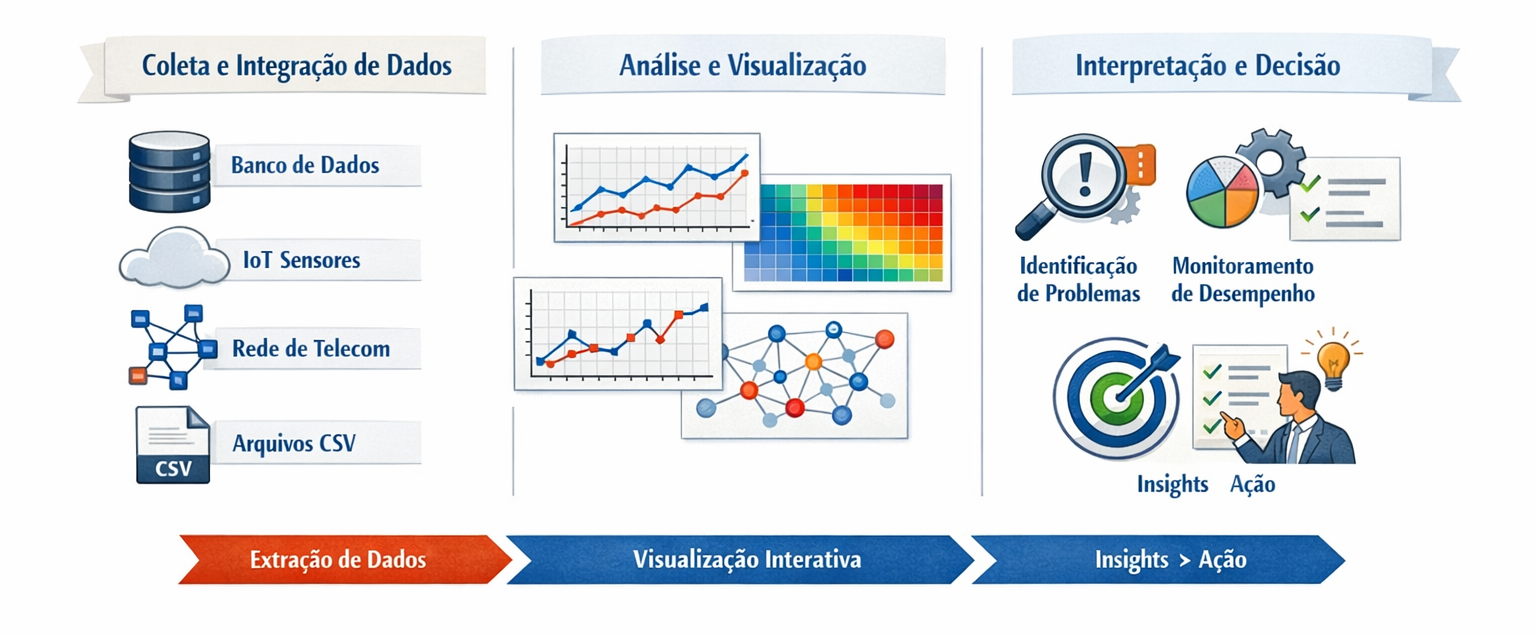
\includegraphics[width=\textwidth]{images/visualizacao_sistemas_complexos.png}
		\par\footnotesize Fonte: Elaboração própria com auxílio de \gls{ia}.
    }
\end{figure}

Conforme ilustrado na Figura~\ref{fig:visualizacao_sistemas_complexos}, o mapeamento de dados em sistemas complexos envolve múltiplas etapas interdependentes, incluindo a coleta e integração de registros provenientes de diferentes fontes, a análise e representação visual dessas informações e, por fim, a interpretação dos resultados para identificação de padrões, geração de \textit{insights} e suporte à tomada de decisão \cite{munzner2014visualization,card1999information}.

Um aspecto particularmente relevante em cenários complexos é a representação de relações, hierarquias e fluxos. Diferentemente de dados independentes, esses casos exigem exibições capazes de evidenciar conexões entre elementos, bem como sua organização em diferentes níveis. Segundo \citeonline{ware2013information}, a percepção humana é especialmente eficiente na identificação de relações espaciais e estruturais quando estas são apresentadas de forma gráfica, o que reforça a importância de representações visuais para o entendimento de topologias e interdependências.

A interatividade constitui um fator determinante para a compreensão desses tipos de sistemas. Interfaces interativas permitem que o usuário explore diferentes níveis de detalhe, alterne entre visões globais e locais, e investigue relações específicas conforme sua necessidade. \citeonline{munzner2014visualization} destaca que abordagens interativas, baseadas nos princípios de foco e contexto, são particularmente eficazes para apoiar a análise de sistemas extensos e hierárquicos, nos quais uma única representação estática dificilmente seria suficiente .

No contexto das redes ópticas \gls{pon}, a complexidade decorre não apenas da quantidade de elementos envolvidos, mas também da forma como eles se conectam logicamente ao longo da rede. A topologia \gls{pon} apresenta uma estrutura hierárquica, com divisões sucessivas do sinal e múltiplos caminhos possíveis entre a central e os usuários finais. A compreensão desse encadeamento lógico é dificultada quando a informação é apresentada exclusivamente em tabelas, planilhas ou visualizações fragmentadas, uma vez que essas abordagens não evidenciam de maneira clara as relações entre os componentes.

A aplicação de princípios de \textit{design} gráfico em cenários complexos torna-se particularmente relevante para o planejamento de redes \gls{pon}. Representações visuais que evidenciem a topologia lógica da rede, aliadas à interatividade, permitem ao projetista compreender o conjunto das ligações, identificar dependências críticas e avaliar o impacto de modificações na estrutura da rede. Conforme apontado por \citeonline{few2012information}, visualizações eficazes devem priorizar clareza, consistência e alinhamento com as tarefas cognitivas do usuário, de modo a apoiar a análise e não apenas a apresentação da informação.

Assim, a representação gráfica, quando aplicada de forma adequada, contribui diretamente para a compreensão de sistemas complexos e para a melhoria do processo decisório. No escopo deste trabalho, esses conceitos fundamentam a adoção de uma abordagem que integra cálculo técnico e visualização interativa da topologia lógica da rede \gls{pon}, visando oferecer ao projetista uma visão mais clara, consistente e abrangente do sistema planejado.

\section{Aplicações Web e Arquitetura Cliente-Servidor}
 
Aplicações web são sistemas de software acessados por meio de um navegador e disponibilizados por uma infraestrutura de rede, permitindo centralizar dados e serviços em um ambiente servidor. Em comparação com aplicações locais, esse modelo reduz dependências do dispositivo do usuário e facilita manutenção e atualização, pois evoluções no servidor tornam-se imediatamente disponíveis aos clientes. Do ponto de vista da engenharia de software, a definição de uma arquitetura clara é essencial para favorecer confiabilidade, manutenibilidade e evolução do sistema ao longo do tempo \cite{pressman2014software,sommerville2016software}.

A organização mais comum para esse tipo de sistema é o modelo cliente-servidor, no qual responsabilidades são distribuídas entre o cliente (interface e interação) e o servidor (processamento, regras de negócio e gerenciamento de dados). Essa separação permite que diferentes tecnologias sejam empregadas em cada parte e contribui para modularidade, reutilização e escalabilidade, uma vez que o servidor pode atender múltiplas requisições simultâneas e ter sua capacidade ampliada por ajustes na infraestrutura \cite{tanenbaum2011networks,pressman2014software}.

O modelo cliente-servidor possibilita a separação entre interface, processamento e armazenamento de dados, contribuindo para a modularidade e a escalabilidade do sistema. A Figura~\ref{fig:cliente_servidor} ilustra essa arquitetura, evidenciando o fluxo de comunicação entre as duas partes por meio de requisições e respostas \cite{tanenbaum2011networks,pressman2014software}.

\begin{figure}[htb]
	\caption{Modelo de arquitetura cliente-servidor, destacando a interação entre cliente e servidor por meio de requisições e respostas em uma rede de comunicação}
	\label{fig:cliente_servidor}
    \centering
    \parbox{16cm}{
		\centering
		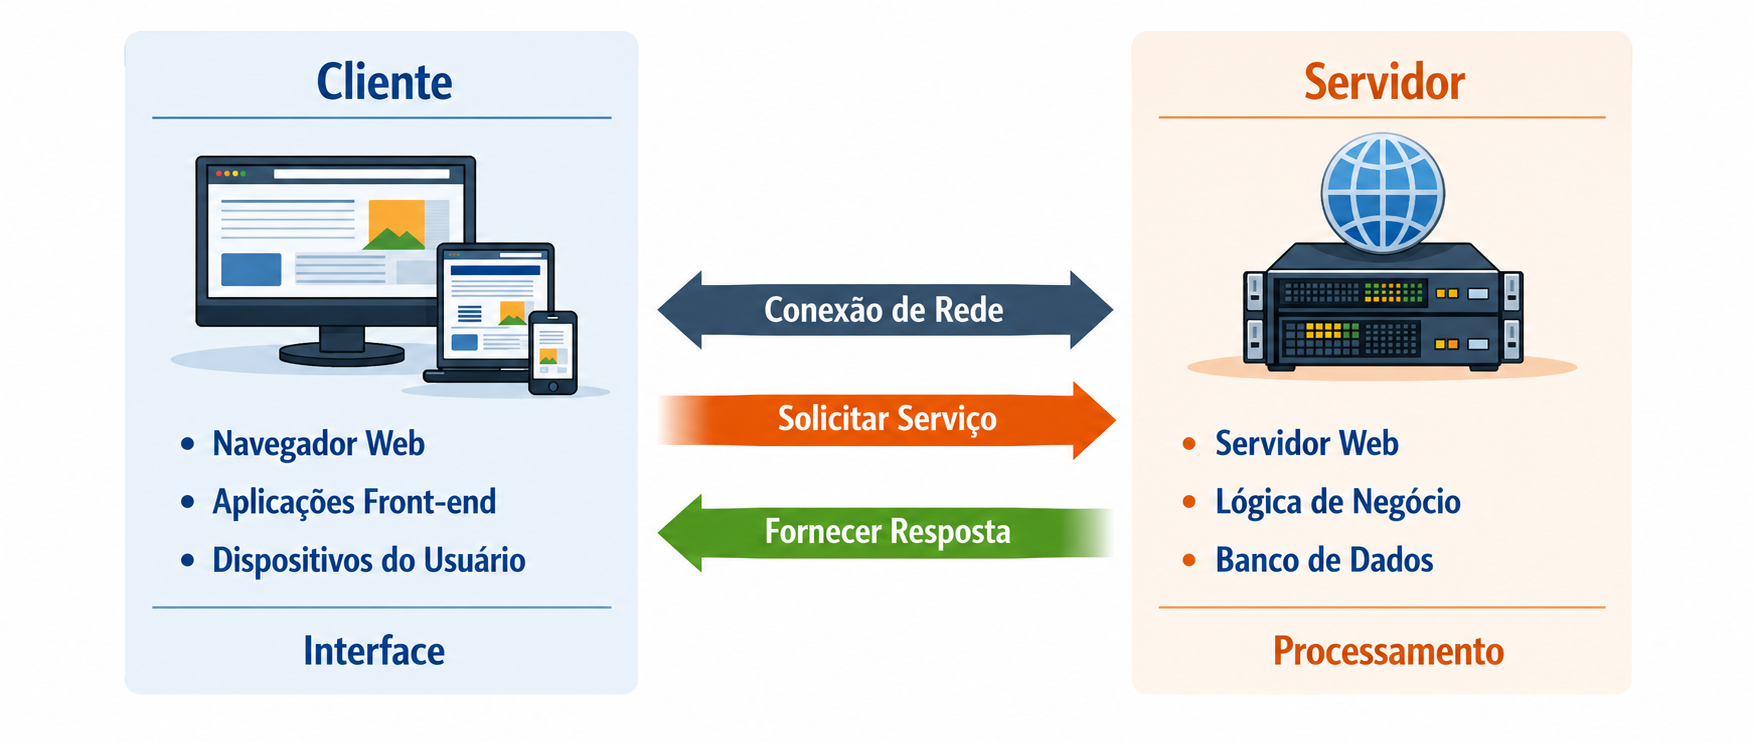
\includegraphics[width=\textwidth]{images/cliente_servidor.png}
		\par\footnotesize Fonte: Elaboração própria com auxílio de \gls{ia}.
    }
\end{figure}

No contexto de aplicações web, essa divisão é frequentemente descrita como \textit{frontend} e \textit{backend}: o \textit{frontend} concentra a camada de apresentação e a experiência do usuário, enquanto o \textit{backend} expõe serviços e recursos e executa validações e operações sobre os dados. Em muitas soluções, essa organização é refinada em uma arquitetura segmentada, separando apresentação, lógica de aplicação e persistência. Ao desacoplar essas responsabilidades, mudanças em um nível tendem a produzir impacto limitado nos demais níveis, reduzindo a complexidade do sistema e facilitando testes, manutenção e atualização \cite{pressman2014software,sommerville2016software}.

A partir dessa base arquitetural, a integração entre cliente e servidor ocorre por meio de interfaces bem definidas (\glspl{api}), usualmente sobre o protocolo \gls{http}, e pode adotar estilos e padrões específicos conforme as necessidades do sistema. Assim, conceitos como \gls{mvc} (para organização interna do \textit{backend}), \gls{rest} (para o estilo de comunicação) e \gls{json} (para representação de dados) complementam o modelo cliente-servidor ao fornecerem mecanismos práticos para estruturar, expor e interoperar funcionalidades e informações em aplicações web distribuídas.

Nesse contexto, a arquitetura cliente-servidor será empregada neste trabalho para estruturar a aplicação web proposta, permitindo separar a interface de modelagem visual da rede das rotinas de cálculo e processamento, favorecendo a organização e a escalabilidade do sistema.

\section{Padrão Arquitetural \gls{mvc}}

O padrão arquitetural \gls{mvc} é amplamente utilizado no desenvolvimento de aplicações como uma forma de organizar o sistema a partir da separação de responsabilidades entre seus componentes. Proposto originalmente por \citeonline{reenskaug1979mvc}, o \gls{mvc} estabelece uma divisão clara entre a representação dos dados, a lógica de controle e a interface com o usuário, contribuindo para a modularidade e a manutenção do software ao longo do tempo.

No padrão \gls{mvc}, o \textit{Model} é responsável pela representação dos dados e pelas regras de negócio da aplicação. Essa camada encapsula a lógica associada ao domínio do problema, incluindo validações, cálculos e estruturas de dados, mantendo-se independente da forma como as informações são apresentadas ao usuário. Essa característica favorece a reutilização e a consistência do comportamento do sistema \cite{pressman2014software}.

A \textit{View} corresponde à camada de apresentação da aplicação, sendo responsável por exibir as informações ao usuário e permitir sua interação com o sistema. No contexto de aplicações web, a \textit{View} é frequentemente implementada por meio de interfaces gráficas executadas no navegador, que consomem dados fornecidos pelos demais componentes do sistema. Ao isolar a apresentação da lógica de negócio, o padrão \gls{mvc} permite que alterações na interface sejam realizadas sem impactar diretamente o processamento interno da aplicação \cite{sommerville2016software}.

O \textit{Controller} atua como intermediário entre o \textit{Model} e a \textit{View}, sendo responsável por receber as requisições do usuário, interpretá-las e acionar as operações apropriadas no \textit{Model}. Após o processamento, o \textit{Controller} coordena a atualização da \textit{View}, garantindo que as informações apresentadas reflitam o estado atual dos dados. Esse papel de mediação contribui para a organização do fluxo de controle da aplicação e para a separação clara das responsabilidades, conforme ilustrado na Figura \ref{fig:mvc} \cite{pressman2014software}.

\begin{figure}[htb]
	\caption{Fluxo de interação do padrão \gls{mvc}}
	\label{fig:mvc}
    \centering
    \parbox{16cm}{
		\centering
		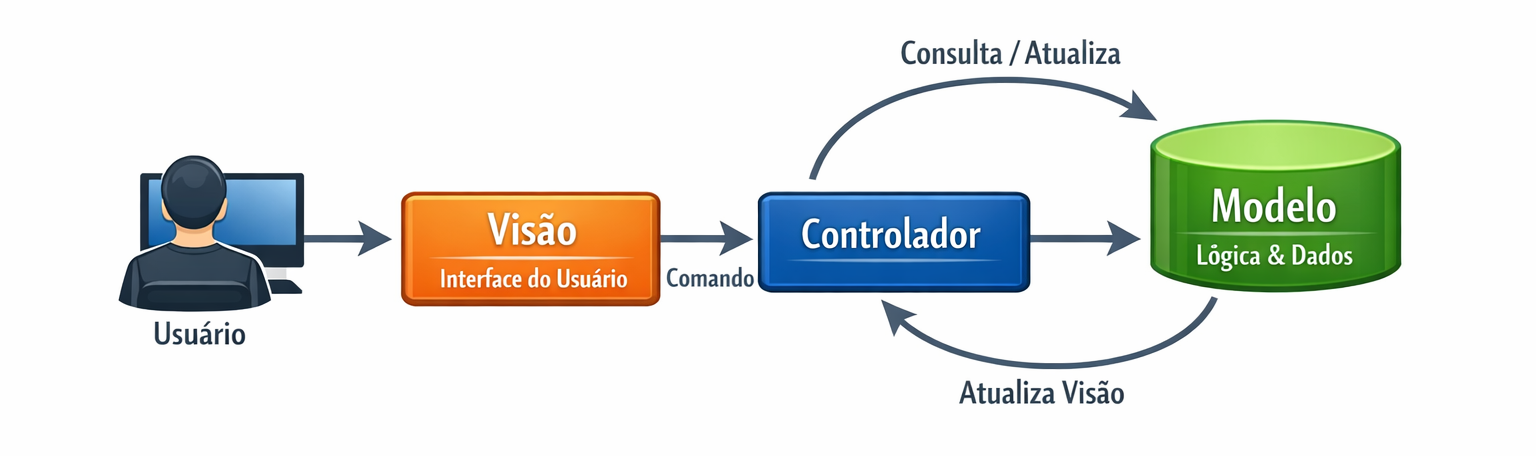
\includegraphics[width=\textwidth]{images/mvc.png}
		\par\footnotesize Fonte: Elaboração própria com auxílio de \gls{ia}.
    }
\end{figure}

\%A utilização do padrão \gls{mvc} em aplicações web favorece a construção de sistemas mais organizados, compreensíveis e extensíveis, especialmente em cenários que envolvem processamento técnico e manipulação de dados estruturados. Ao separar a lógica de negócio da interface e do controle de fluxo, o \gls{mvc} estabelece uma base arquitetural adequada para a integração com outros estilos e tecnologias, como serviços web e interfaces interativas, contribuindo para a evolução consistente da aplicação ao longo do tempo.

Dessa forma, o padrão \gls{mvc} será adotado na organização do \textit{backend} da aplicação, permitindo separar a lógica de cálculo do orçamento óptico, o controle das requisições e a manipulação dos dados, contribuindo para a clareza, manutenção e escalabilidade do sistema desenvolvido.

\section{Comunicação Web: \gls{http} e \glspl{api}}

A comunicação entre componentes em aplicações web baseia-se, de forma predominante, em mecanismos padronizados que permitem a troca de informações entre clientes e servidores distribuídos em rede. No contexto do modelo cliente-servidor, essa comunicação é realizada por meio de protocolos que definem como as requisições são enviadas, como as respostas são estruturadas e como os dados são transmitidos de forma confiável. Entre esses protocolos, destaca-se o \gls{http}, amplamente adotado como base para a comunicação em aplicações web modernas \cite{tanenbaum2011networks}.

O protocolo \gls{http} define um modelo de comunicação do tipo requisição-resposta, no qual o cliente envia uma solicitação ao servidor e aguarda o retorno de uma resposta correspondente. Cada requisição contém informações que identificam o recurso desejado e o tipo de operação a ser realizada, enquanto a resposta do servidor inclui os dados solicitados ou o resultado do processamento, além de códigos de \textit{status} que indicam o sucesso ou falha da comunicação. Esse modelo simples e padronizado contribui para a interoperabilidade entre sistemas heterogêneos e para a ampla adoção do \gls{http} em ambientes distribuídos \cite{tanenbaum2011networks}.

No desenvolvimento de soluções web, o uso do \gls{http} é frequentemente associado ao conceito de \glspl{api}. Uma \gls{api} pode ser entendida como um conjunto de interfaces e regras que permitem a troca de informações entre diferentes componentes de software, definindo como funcionalidades e dados podem ser acessados de forma controlada. Em aplicações baseadas em arquitetura cliente-servidor, as \glspl{api} desempenham papel fundamental ao estabelecer um ponto de comunicação bem definido entre o \textit{frontend} e o \textit{backend}, promovendo o desacoplamento entre a interface do usuário e a lógica de processamento, conforme ilustrado na Figura~\ref{fig:http_api} \cite{sommerville2016software}.

\begin{figure}[htb]
	\caption{Comunicação entre cliente e servidor por meio de \gls{http} e \gls{api}}
	\label{fig:http_api}
    \centering
    \parbox{16cm}{
		\centering
		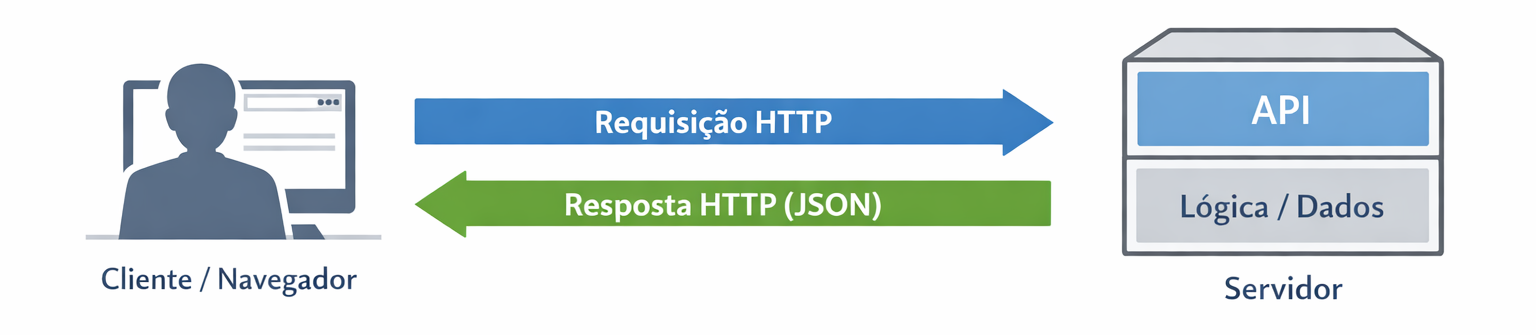
\includegraphics[width=\textwidth]{images/http_api.png}
		\par\footnotesize Fonte: Elaboração própria com auxílio de \gls{ia}.
    }
\end{figure}

A adoção de \glspl{api} na comunicação web contribui para a modularidade e a extensibilidade das aplicações, uma vez que diferentes clientes podem consumir os mesmos serviços oferecidos pelo servidor, desde que respeitem as interfaces estabelecidas. Essa abordagem facilita a evolução do sistema, possibilita a integração com outros serviços e reduz a dependência direta entre os componentes da aplicação. Conforme discutido na literatura de engenharia de software, interfaces bem definidas são essenciais para o desenvolvimento de sistemas distribuídos mais organizados, reutilizáveis e de fácil manutenção \cite{pressman2014software}.

O uso do protocolo \gls{http} em conjunto com \glspl{api} constitui a base da comunicação em aplicações web modernas, permitindo a troca estruturada de informações entre clientes e servidores. Essa combinação estabelece o fundamento sobre o qual estilos arquiteturais específicos de comunicação são construídos, viabilizando a implementação de soluções distribuídas escaláveis e interoperáveis.

Assim, a comunicação via \gls{http} será empregada neste trabalho como base para a troca de dados entre os componentes da aplicação, garantindo a interoperabilidade entre a interface web e os serviços responsáveis pelo processamento dos cálculos.


\section{\gls{api} \textit{RESTful}}

O estilo arquitetural \gls{rest} foi proposto por \citeonline{fielding2000rest} como um conjunto de princípios para a construção de sistemas distribuídos baseados em rede, com foco em escalabilidade, simplicidade e baixo acoplamento entre os componentes. No contexto das aplicações web, o \gls{rest} consolidou-se como uma abordagem amplamente adotada para o desenvolvimento de \glspl{api}, sendo utilizado como base para a comunicação entre clientes e servidores em sistemas cliente-servidor modernos.

Uma \gls{api} \textit{RESTful} organiza a comunicação em torno do conceito de recursos, que representam entidades ou conjuntos de dados manipulados pelo sistema. Cada recurso é identificado de forma única por meio de uma \gls{uri} e pode ser acessado ou manipulado por operações padronizadas. Essas operações são realizadas utilizando os métodos definidos pelo protocolo \gls{http}, o que permite explorar mecanismos amplamente suportados pela infraestrutura da web \cite{fielding2000rest}

Entre os princípios fundamentais do \gls{rest} destaca-se a característica \textit{stateless}, segundo a qual cada requisição enviada pelo cliente ao servidor deve conter todas as informações necessárias para seu processamento. O servidor não mantém estado da sessão do cliente entre requisições, o que contribui para a escalabilidade do sistema e simplifica o gerenciamento das interações. Essa abordagem reduz dependências entre requisições consecutivas e facilita a distribuição da carga de processamento entre diferentes instâncias servidoras, conforme ilustrado na Figura~\ref{fig:api_restfull} \cite{fielding2000rest}.

\begin{figure}[htb]
	\caption{Estrutura conceitual de uma \gls{api} \textit{RESTful}}
	\label{fig:api_restfull}
    \centering
    \parbox{16cm}{
		\centering
		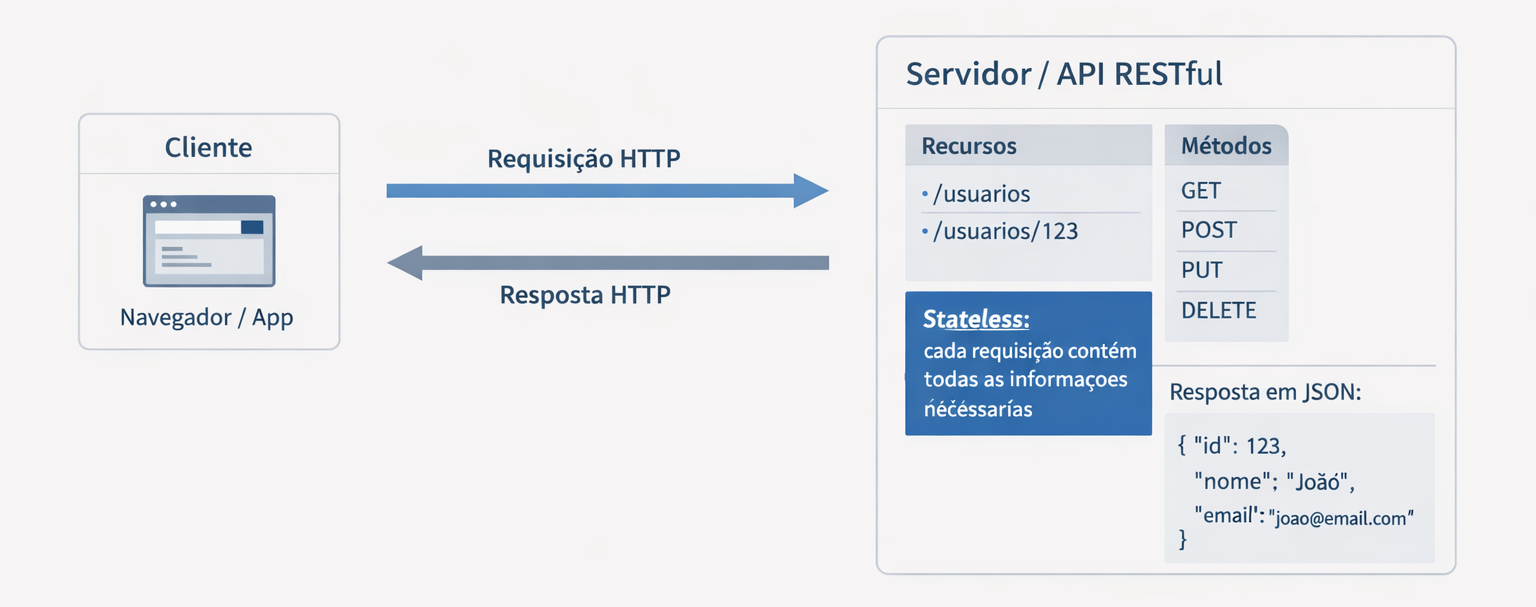
\includegraphics[width=\textwidth]{images/api_restfull.png}
		\par\footnotesize Fonte: Elaboração própria com auxílio de \gls{ia}.
    }
\end{figure}

A adoção do estilo \gls{rest} em aplicações web contribui para a construção de sistemas mais organizados, interoperáveis e extensíveis. Ao basearem a comunicação em princípios bem definidos e amplamente aceitos, as \glspl{api} \textit{RESTful} estabelecem uma infraestrutura de comunicação adequada para aplicações distribuídas que demandam integração entre múltiplos componentes, servindo como base para o intercâmbio estruturado de dados e para a implementação de serviços web modernos \cite{fielding2000rest}.

Nesse contexto, a adoção de uma \gls{api} \textit{RESTful} neste projeto permite estruturar a comunicação entre o \textit{frontend} e o \textit{backend} de forma modular e padronizada, facilitando o envio de dados da topologia da rede e o retorno dos resultados do cálculo do orçamento óptico.

\section{Formato de Intercâmbio de Dados: \gls{json}}

Em aplicações web modernas, a troca de informações entre cliente e servidor requer o uso de formatos de dados padronizados, capazes de representar estruturas de informação de forma clara, eficiente e independente de plataforma. No contexto de \gls{api} \textit{RESTful}, esses formatos desempenham papel essencial, pois viabilizam o intercâmbio estruturado de dados entre diferentes componentes do sistema, garantindo interoperabilidade e consistência na comunicação.

O \gls{json} é um formato leve de representação de dados, baseado em texto, amplamente utilizado em aplicações web e serviços baseados em \gls{http}. Definido originalmente como uma notação derivada da linguagem JavaScript, o \gls{json} consolidou-se como um formato independente de linguagem, sendo suportado por diversas plataformas e ambientes de desenvolvimento. Sua estrutura baseia-se em pares chave-valor e em listas ordenadas, permitindo a representação de dados simples e complexos de maneira hierárquica e legível, conforme ilustrado na Figura~\ref{fig:json_estrutura} \cite{bray2017json}.

\begin{figure}[htb]
	\caption{Estrutura conceitual do formato \gls{json}}
	\label{fig:json_estrutura}
    \centering
    \parbox{16cm}{
		\centering
		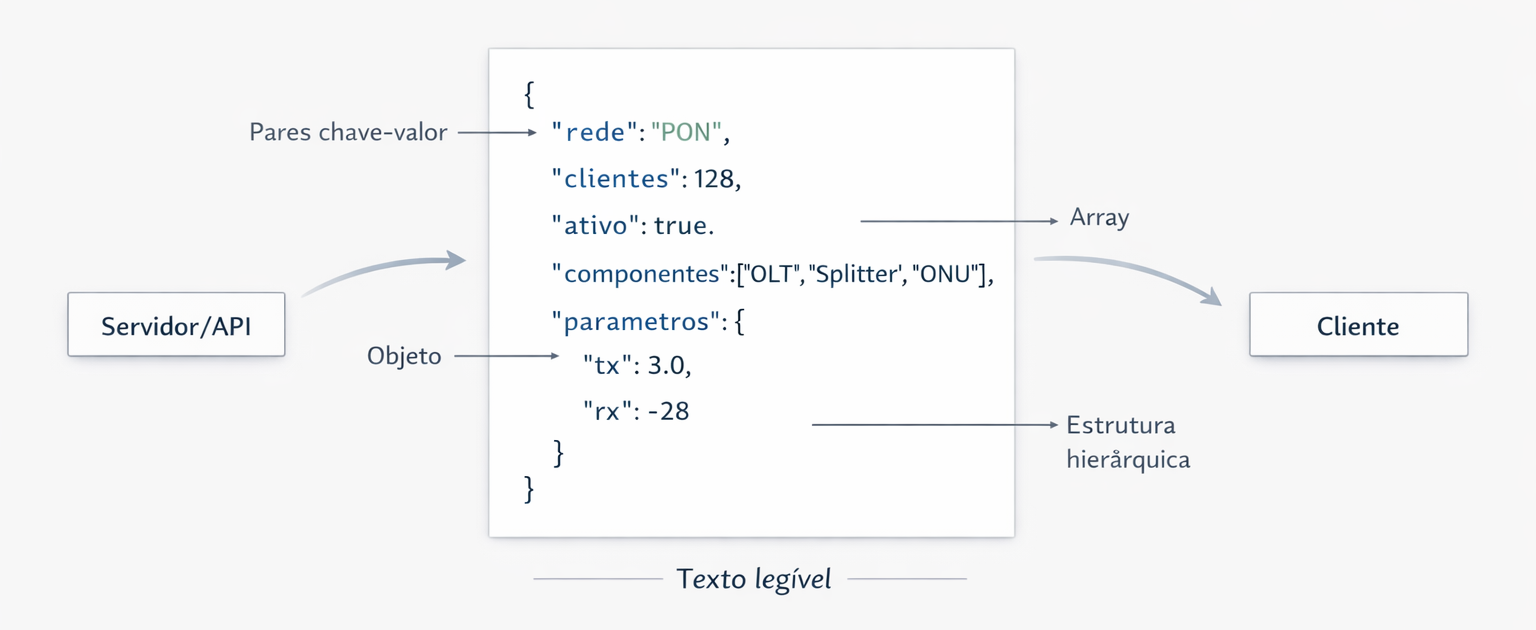
\includegraphics[width=\textwidth]{images/json_estrutura.png}
		\par\footnotesize Fonte: Elaboração própria com auxílio de \gls{ia}.
    }
\end{figure}

Uma das principais características do \gls{json} é sua simplicidade sintática, que facilita tanto a leitura humana quanto o processamento automático pelos sistemas. Em comparação com formatos mais verbosos, como XML, o \gls{json} apresenta menor sobrecarga de dados, contribuindo para a redução do volume de informações enviadas pela rede e para a melhoria do desempenho das aplicações distribuídas. Essas características tornam o \gls{json} particularmente adequado para a comunicação em \glspl{api} \textit{RESTful}, nas quais eficiência e clareza na troca de dados são requisitos relevantes \cite{bray2017json}.

No contexto da arquitetura cliente-servidor, o uso do \gls{json} como formato de intercâmbio assegura a neutralidade tecnológica na transmissão, uma vez que os dados terão representação neutra, independente das tecnologias utilizadas em cada componente. Dessa forma, o servidor pode fornecer informações estruturadas por meio de respostas \gls{http}, enquanto o cliente interpreta e utiliza esses dados conforme suas necessidades de apresentação ou interação, sem dependência direta da implementação interna do servidor \cite{sommerville2016software}.

Além de seu uso na comunicação entre componentes, o \gls{json} também é amplamente empregado para o armazenamento e a serialização de dados estruturados em aplicações web. Sua flexibilidade permite representar configurações, estados e estruturas complexas de informação de forma organizada e facilmente manipulável. Assim, o \gls{json} estabelece-se como um elemento fundamental na infraestrutura de aplicações web modernas, servindo como base para a troca de dados em sistemas distribuídos e integrados.

Dessa forma, o formato \gls{json} será utilizado neste trabalho para representar a topologia da rede óptica, permitindo o armazenamento estruturado dos elementos e sua fácil integração com a visualização interativa implementada com a biblioteca D3.js.

\section{Visualização de Dados em Aplicações Web}

A visualização de dados constitui um elemento fundamental em sistemas computacionais que lidam com grandes volumes de informações ou com estruturas de dados complexas. Seu objetivo principal é transformar dados abstratos em representações visuais que facilitem a compreensão, a análise e a interpretação das informações, apoiando processos de tomada de decisão. Em aplicações web, a visualização assume papel ainda mais relevante, uma vez que a interface gráfica representa o principal meio de interação entre o usuário e os dados processados pelo sistema \cite{card1999information,ware2013information}.

Em sistemas baseados em arquitetura cliente-servidor, a visualização de dados está geralmente associada à camada de apresentação da aplicação, sendo responsável por representar, de forma gráfica, as informações fornecidas pelo \textit{backend}. Essa separação permite que o processamento e a organização dos dados ocorram no servidor, enquanto o cliente se encarrega de exibir essas informações de maneira adequada ao usuário. A utilização de visualizações gráficas contribui para reduzir a carga cognitiva associada à interpretação de dados complexos, tornando explícitas relações, hierarquias e padrões que seriam difíceis de identificar por meio de representações puramente textuais ou tabulares \cite{card1999information}.

As aplicações web modernas demandam visualizações que vão além da simples apresentação estática de informações. A interatividade passou a ser um requisito importante, permitindo que o usuário explore os dados, alterne entre diferentes níveis de detalhe e observe o impacto de modificações nos parâmetros de entrada. Conforme discutido na literatura, visualizações interativas ampliam a capacidade de análise ao combinar representações gráficas com mecanismos de exploração, favorecendo a compreensão de sistemas complexos e dinâmicos, conforme ilustrado na Figura~\ref{fig:visualizacao_web} \cite{munzner2014visualization}.

\begin{figure}[htb]
	\caption{Visualização interativa de dados em aplicações web}
	\label{fig:visualizacao_web}
    \centering
    \parbox{16cm}{
		\centering
		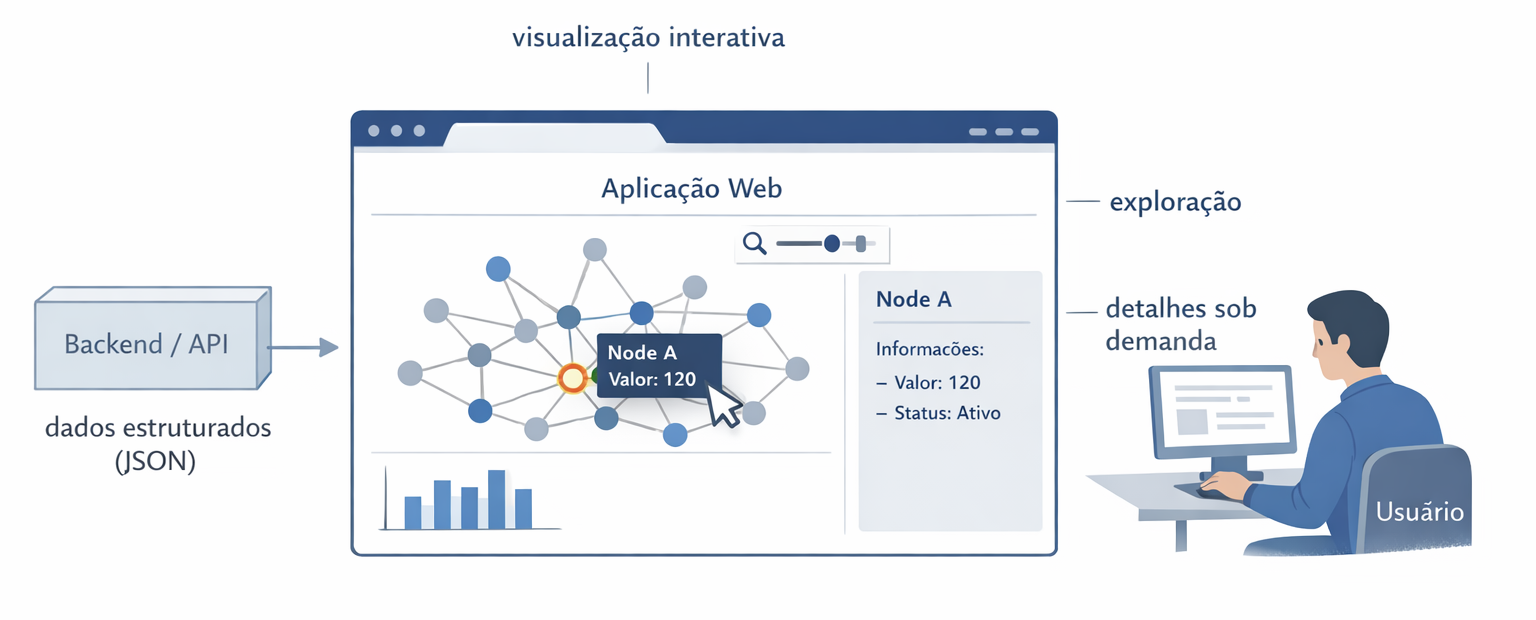
\includegraphics[width=\textwidth]{images/visualizacao_web.png}
		\par\footnotesize Fonte: Elaboração própria com auxílio de \gls{ia}.
    }
\end{figure}

Outro aspecto relevante da visualização de dados em aplicações web é sua integração com dados estruturados provenientes de \glspl{api} e serviços distribuídos. Formatos de intercâmbio como o \gls{json} permitem que informações organizadas sejam transmitidas do servidor para o cliente, onde podem ser processadas e representadas visualmente de forma dinâmica. Essa integração entre dados estruturados e visualização gráfica reforça o papel da visualização como componente essencial na construção de aplicações web voltadas à análise e ao planejamento \cite{sommerville2016software}.

Dessa forma, a visualização de dados em aplicações web constitui um recurso indispensável para a representação clara e eficiente de informações técnicas e estruturadas. Ao permitir a exploração visual dos dados e a interação direta do usuário com as informações apresentadas, as visualizações contribuem para a compreensão global do sistema e para a melhoria da experiência de uso, estabelecendo a base conceitual para o emprego de bibliotecas especializadas em visualização gráfica no ambiente web.

\section{Biblioteca D3.js para Visualização Interativa}

No contexto das aplicações web, a implementação de visualizações interativas demanda o uso de bibliotecas especializadas capazes de transformar dados estruturados em representações gráficas dinâmicas. Entre as ferramentas disponíveis para esse fim, destaca-se a biblioteca D3.js (\textit{Data-Driven Documents}), amplamente utilizada para a criação de visualizações personalizadas e orientadas a dados no ambiente web \cite{bostock2011d3}.

A D3.js baseia-se no princípio de vincular dados diretamente aos elementos do documento, permitindo que mudanças nos dados sejam refletidas automaticamente na representação visual. Essa abordagem orientada a dados possibilita a construção de visualizações altamente flexíveis, nas quais atributos gráficos como posição, cor, forma e tamanho podem ser definidos a partir dos valores dos dados subjacentes. Diferentemente de bibliotecas que oferecem apenas componentes gráficos pré-definidos, a D3.js fornece mecanismos de baixo nível que permitem maior controle sobre a estrutura e o comportamento das visualizações, conforme ilustrado na Figura~\ref{fig:d3js_conceito} \cite{bostock2011d3}.

\begin{figure}[htb]
	\caption{Transformação de dados em elementos visuais interativos com D3.js}
	\label{fig:d3js_conceito}
    \centering
    \parbox{16cm}{
		\centering
		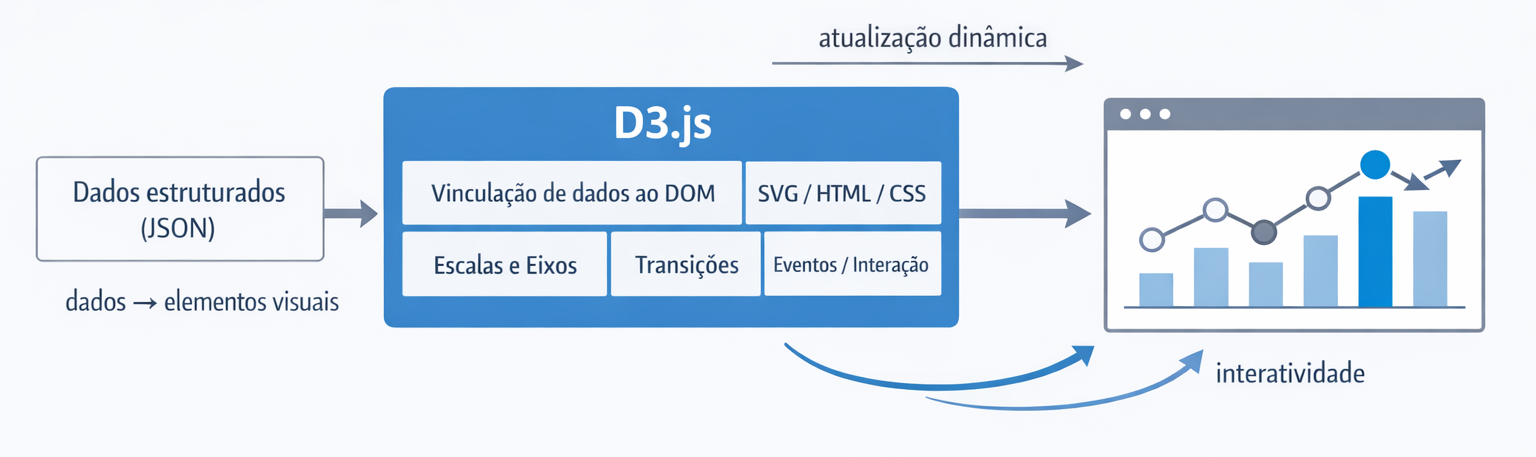
\includegraphics[width=\textwidth]{images/d3js_conceito.png}
		\par\footnotesize Fonte: Elaboração própria com auxílio de \gls{ia}.
    }
\end{figure}

Outro aspecto relevante da D3.js é sua integração nativa com tecnologias fundamentais da web, como \gls{html}, \gls{svg} e \gls{css}. Essa integração permite que as visualizações façam parte da estrutura do documento web, favorecendo a criação de interfaces ricas e interativas sem a necessidade de ambientes gráficos proprietários ou extensões específicas. Além disso, a utilização de padrões abertos contribui para a portabilidade e a compatibilidade das visualizações em diferentes navegadores e dispositivos \cite{bostock2011d3}.

A D3.js também oferece suporte à interatividade, possibilitando a implementação de mecanismos como atualização dinâmica dos dados, animações, transições e respostas a eventos de interação do usuário. Esses recursos são particularmente importantes em aplicações que envolvem a exploração de dados complexos, pois permitem que o usuário investigue diferentes aspectos da informação apresentada, altere parâmetros e observe, em tempo real, os efeitos dessas alterações sobre a visualização \cite{munzner2014visualization}.

A adoção da biblioteca D3.js em aplicações voltadas à visualização de dados proporciona uma base adequada para a representação gráfica interativa de informações técnicas e estruturadas. Ao combinar flexibilidade, integração com padrões web e suporte à interatividade, a D3.js constitui uma ferramenta apropriada para a construção de visualizações que auxiliam na compreensão e na análise de sistemas complexos, especialmente em contextos que demandam clareza na representação da estrutura e do comportamento dos dados.

Nesse sentido, a biblioteca D3.js será utilizada neste projeto para a construção da visualização interativa da topologia da rede, permitindo representar graficamente os elementos e suas conexões, além de atualizar dinamicamente os resultados do orçamento óptico conforme as alterações realizadas pelo usuário.


\section{Execução e Implantação de Aplicações Web (\textit{Docker})}

A execução e a implantação de aplicações web envolvem a definição de um ambiente computacional capaz de suportar corretamente os componentes do sistema, incluindo dependências de software, bibliotecas e configurações necessárias para seu funcionamento. Em aplicações distribuídas, diferenças entre ambientes de desenvolvimento, teste e produção podem introduzir inconsistências que afetam a confiabilidade e a reprodutibilidade do sistema. Nesse contexto, abordagens que visam padronizar o ambiente de execução tornam-se relevantes para a estabilidade e a manutenção das aplicações web.

A conteinerização surge como uma solução para esse problema ao permitir o empacotamento da aplicação e de todas as suas dependências em unidades isoladas, conhecidas como contêineres. Diferentemente de abordagens baseadas em virtualização completa, os contêineres compartilham o núcleo do sistema operacional hospedeiro, oferecendo um ambiente leve e eficiente para a execução de aplicações. Essa característica contribui para a portabilidade do sistema, possibilitando que a aplicação seja executada de forma consistente em diferentes plataformas e infraestruturas \cite{pahl2015containerization}.

O \textit{Docker} é uma das ferramentas mais difundidas para a implementação do modelo de conteinerização, sendo amplamente adotado no desenvolvimento e na implantação de aplicações web. Por meio do \textit{Docker}, torna-se possível definir ambientes de execução padronizados, nos quais a aplicação e seus serviços associados operam de maneira isolada do sistema hospedeiro. Essa padronização reduz dependências externas, simplifica o processo de execução e facilita a replicação do ambiente em diferentes contextos, conforme ilustrado na Figura~\ref{fig:docker_implantacao} \cite{merkel2014docker}.

\begin{figure}[htb]
	\caption{Execução de aplicações web em contêineres \textit{Docker}}
	\label{fig:docker_implantacao}
    \centering
    \parbox{16cm}{
		\centering
		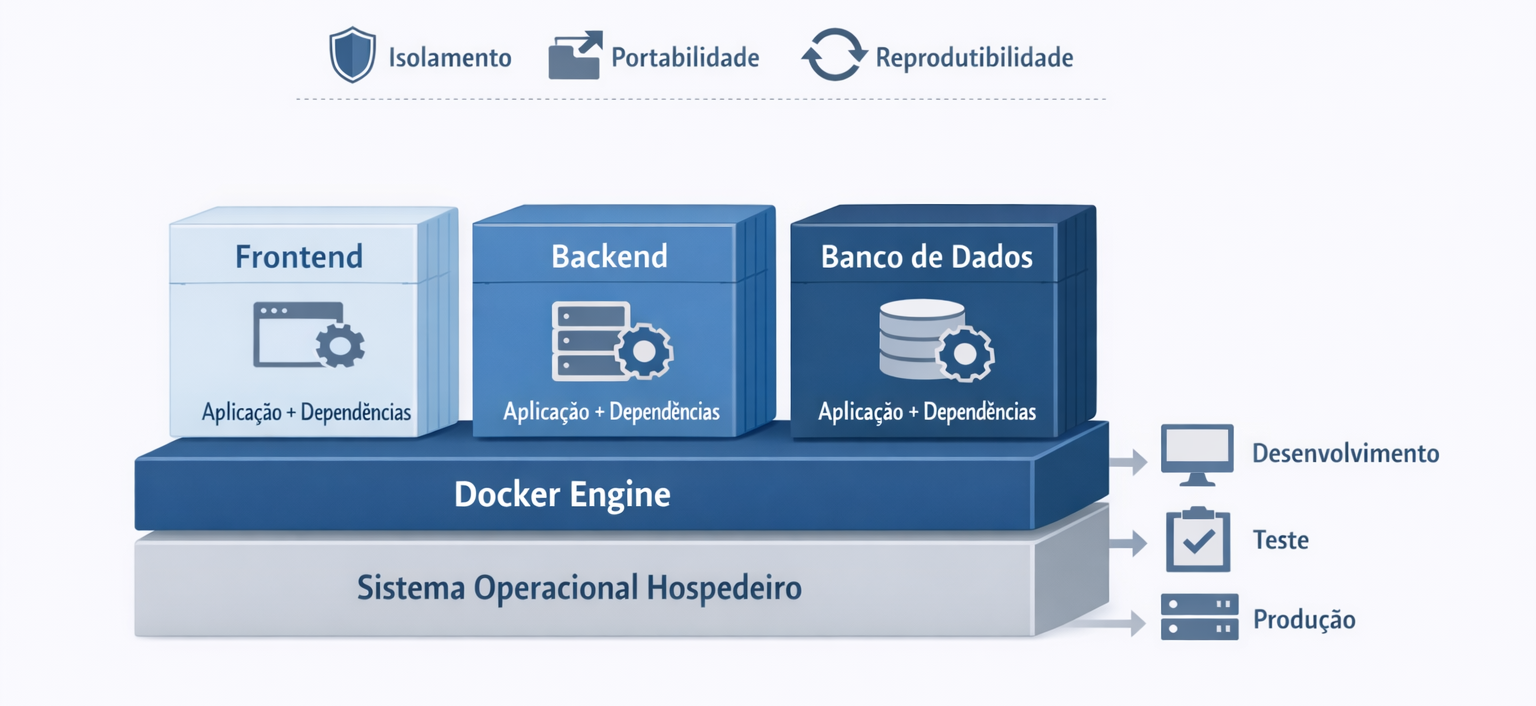
\includegraphics[width=\textwidth]{images/docker_implantacao.png}
		\par\footnotesize Fonte: Elaboração própria com auxílio de \gls{ia}.
    }
\end{figure}

No contexto de aplicações web baseadas em arquitetura cliente-servidor, o uso de contêineres favorece a separação entre os diferentes componentes do sistema, como \textit{frontend} e \textit{backend}, permitindo que cada parte seja executada em um ambiente controlado e consistente. Além disso, a conteinerização contribui para a organização do processo de implantação, uma vez que a aplicação pode ser distribuída e executada de forma uniforme, independentemente do ambiente subjacente.
 
Assim, o \textit{Docker} será utilizado neste trabalho como ferramenta de apoio ao desenvolvimento, permitindo a criação de um ambiente de execução padronizado para a aplicação. Essa abordagem garante que as rotinas de cálculo do orçamento óptico e os serviços da \gls{api} possam ser executados de forma consistente em diferentes ambientes, além de facilitar a posterior implantação do sistema.
